% !TEX program = lualatex
\documentclass[a4paper,11pt]{ltjsarticle}

% ===== フォント設定 =====
\usepackage{luatexja-fontspec}
\setmainjfont{Noto Serif CJK JP}
\setsansjfont{Noto Sans CJK JP}

% ===== パッケージ =====
\usepackage{amsmath}
\usepackage{booktabs}
\usepackage{tikz}
\usepackage{pgfplots}
\pgfplotsset{compat=1.18}
\usepackage[colorlinks=true,linkcolor=blue!60!black,citecolor=green!50!black,urlcolor=blue!70!black]{hyperref}
\usepackage{listings}
\usepackage{xcolor}
\usepackage{graphicx}
\usepackage{longtable}
\usepackage{float}
\usepackage{enumitem}

% ===== TikZライブラリ =====
\usetikzlibrary{arrows.meta, positioning, shapes.geometric, fit, calc, backgrounds, decorations.pathreplacing}

% ===== listings設定 =====
\definecolor{codebg}{RGB}{248,248,248}
\definecolor{codegreen}{RGB}{40,160,40}
\definecolor{codegray}{RGB}{128,128,128}
\definecolor{codeblue}{RGB}{40,40,200}
\definecolor{codestring}{RGB}{163,21,21}

\lstset{
  backgroundcolor=\color{codebg},
  basicstyle=\ttfamily\small,
  breaklines=true,
  captionpos=b,
  commentstyle=\color{codegreen},
  keywordstyle=\color{codeblue}\bfseries,
  stringstyle=\color{codestring},
  numbers=left,
  numberstyle=\tiny\color{codegray},
  numbersep=5pt,
  frame=single,
  framesep=5pt,
  xleftmargin=15pt,
  framexleftmargin=15pt,
  showstringspaces=false,
  tabsize=2,
}

\lstdefinelanguage{R}{
  morekeywords={library,function,if,else,for,while,return,TRUE,FALSE,NULL,
    phil_read,phil_explore,phil_compare,phil_plot,phil_embed,phil_annotate,
    phil_search,phil_align,phil_trace,phil_to_latex,phil_dashboard,
    phil_quantify,phil_segment,phil_lookup,phil_review,phil_tag,
    phil_to_bibtex,phil_export,phil_save,phil_session,phil_config,
    PhilCorpus,ConceptSpans,PhilCollection,
    phil_engine,phil_compare_backends,
    select,keys,columns,tradition_tree,query,
    layers,segmentData,textMetadata,conceptSpans,interpretations},
  sensitive=true,
  morecomment=[l]{\#},
  morestring=[b]",
  morestring=[b]',
}

\lstdefinelanguage{Python}{
  morekeywords={class,def,import,from,return,self,None,True,False,
    Protocol,dataclass,field,Optional,list,dict,tuple,
    PhilCorpus,ConceptSpans,PhilCollection,PhilEngine,
    EmbeddingBackend,FacetedEmbedding,EmbeddingConfig,
    SemanticAlignment,StructuralAlignment,ArgumentativeAlignment,HybridAlignment,
    SchoolClassifier,ArgumentExtractor,InterpretationTracker,
    PhilGraph,EdgeType,NodeBase},
  sensitive=true,
  morecomment=[l]{\#},
  morestring=[b]",
  morestring=[b]',
}

% ===== レイアウト調整 =====
\usepackage{geometry}
\geometry{top=25mm, bottom=25mm, left=25mm, right=25mm}

% ===== 参考文献用 =====
% bibliography uses thebibliography environment

% ===== タイトル =====
\title{{\LARGE Phil Ecosystem:\\
哲学研究のための計算基盤エコシステムの設計と実装}}
\author{松井佑介\thanks{Email: matsui@example.ac.jp}}
\date{}

\begin{document}
\maketitle

\begin{abstract}
哲学研究における計算的手法の導入は、言語学や歴史学と比較して著しく遅れている。
その根本的原因は、哲学固有の課題——概念の通約不可能性、解釈の多重性、
テキストの多言語性（2500年のスパンにわたるギリシャ語・漢文・サンスクリット語・現代諸語）、
そして形式化に対する文化的抵抗——にある。
本論文では、これらの課題に正面から向き合いつつ、哲学研究に計算的アプローチを
「日常化」するためのエコシステム Phil Ecosystem の設計と実装を報告する。

Phil Ecosystem は、生物情報学における Bioconductor の成功パターンに学び、
7層アーキテクチャ（計算バックエンド、リポジトリ、アノテーション、定量化エンジン、
コアデータ構造、専門分析、統合ワークベンチ）を採用する。
中核となるデータコンテナ PhilCorpus は、Bioconductor の SummarizedExperiment を
哲学データに適応させたものであり、テキスト・埋め込み・特徴量の多層構造に加え、
哲学固有の「解釈の多重性」次元を第一級オブジェクトとして組み込む。
研究者は約15の「動詞」（\texttt{phil\_read}, \texttt{phil\_explore},
\texttt{phil\_compare}, \texttt{phil\_plot}等）のみで全機能にアクセスでき、
内部の7層構造を意識する必要がない。

R/Python二言語戦略により、デジタル・ヒューマニティーズ研究者と
機械学習研究者の双方に自然なインターフェースを提供する。
哲学ドメイン特化のファインチューニング済み埋め込みモデル（philmap-e5-v2,
Spearman $\rho = 0.976$）により、和辻の「間柄」からハイデガーの Mitsein、
ブーバーの Ich-Du、ウブントゥ哲学まで、言語・伝統を超えた概念検索を実現する。
本エコシステムは、「計算が哲学に対して、望遠鏡が天文学に対して果たした役割を
果たす」というビジョンのもと、個人の認知限界を超えた哲学研究の新たな
パラダイムを構築することを目指す。

\medskip
\noindent\textbf{キーワード:}
デジタル・ヒューマニティーズ, 計算哲学, 比較哲学, 概念整列,
多言語埋め込み, 知識グラフ, ソフトウェアエコシステム
\end{abstract}

\tableofcontents
\newpage

%% ==========================================================================
%% 第1章 はじめに
%% ==========================================================================
\section{はじめに}\label{sec:intro}

\subsection{哲学研究における情報技術導入の現状}

21世紀に入り、人文学の諸分野は情報技術との融合を急速に進めてきた。
言語学では大規模コーパスに基づく統計的手法が標準的方法論となり、
歴史学では GIS（地理情報システム）やテキストマイニングによるデジタル・アーカイブの
構築が進んでいる。考古学ではフォトグラメトリやライダー（LiDAR）による
三次元記録が不可欠な技術となった。
文学研究においても、Franco Moretti の「遠読（distant reading）」\cite{moretti2013}
以降、計算的テキスト分析は広く受容されつつある。

しかし、哲学研究は他の人文学分野と比較して、計算的手法の導入が顕著に遅れている。
PhilPapers\cite{bourget2014} や InPhO（Indiana Philosophy Ontology）\cite{niepert2008}
のような知識基盤は存在するものの、これらは哲学研究の「道具」というよりも
「資料索引」にとどまっている。哲学者の日常的な研究——テキストの精読、
概念の比較、論証の分析——に計算的手法が統合されている事例はきわめて少ない。

\subsection{他の人文学との比較：なぜ哲学は遅れているのか}

この遅れには構造的な理由がある。
第一に、哲学が扱うデータは本質的に「解釈を要する」ものであり、
テキストの統計的処理が直ちに哲学的洞察につながるわけではない。
語の出現頻度を数えても、カントの超越論的演繹の構造は見えてこない。
この点で、哲学は言語学の統計的アプローチとは異なる方法論を必要とする。

第二に、哲学テキストの言語的多様性は他分野と比較しても際立っている。
古典ギリシャ語、ラテン語、サンスクリット語、漢文、アラビア語、
そして現代の英語・ドイツ語・フランス語・日本語など、
2500年以上のスパンにわたる多言語テキストを横断的に扱う必要がある。
歴史学も多言語テキストを扱うが、特定の時代・地域に限定されることが多い。
哲学では、紀元前5世紀のギリシャのテキストと20世紀の日本のテキストを
同じ概念的枠組みで比較するという要求が日常的に生じる。

第三に、そしておそらく最も本質的な理由として、
哲学者コミュニティには形式化に対する根深い懐疑がある。
概念の計算的処理は、概念の豊かさの「矮小化」と見なされがちである。
ハイデガーの Dasein をベクトルに変換することに、
現象学者が抵抗を感じるのは自然なことかもしれない。
しかし、これは望遠鏡の導入に対して
「肉眼で見えないものは天体ではない」と主張するようなものでもある。

\subsection{本エコシステムのビジョン}

本論文で提案する Phil Ecosystem は、次のビジョンに基づいている：

\begin{quote}
\textit{計算は哲学に対して、望遠鏡が天文学に対して果たしたのと同じ役割を果たせるか？}
\end{quote}

望遠鏡は「肉眼では見えなかったもの」を見えるようにし、天文学のパラダイムを変えた。
ガリレオが木星の衛星を発見したとき、それは望遠鏡なしでは原理的に不可能な発見であった。
同様に、Phil Ecosystem は「いかなる個人の読解でも到達できなかった概念間の関係」を
計算的に可視化することを目指す。

例えば、和辻哲郎の「間柄」概念と南アフリカのウブントゥ哲学における
「umuntu ngumuntu ngabantu（人は他の人々を通じてこそ人である）」という命題の間に、
構造的な類似性はあるだろうか。
この問いに答えるには、日本語とズールー語の両方を読める哲学者が必要であるが、
そのような研究者はほぼ存在しない。
計算的アプローチは、この「個人の言語能力の限界」という構造的制約を超える
可能性を持つ。もちろん、計算が「発見」するのは類似性の候補であり、
その哲学的意義の評価は依然として人間の仕事である。
しかし、候補の発見すらなければ、評価も始まらない。

\subsection{論文の構成}

本論文は、異なる読者層を意識して前半と後半に分かれている。

前半（第2章--第6章）は主に哲学研究者を対象とし、
計算的アプローチの必要性（第2章）、日常化のための設計思想（第3章）、
具体的な利用事例（第4章）、データ構造の概要（第5章）を平易に説明する。
哲学研究者がこの部分だけを読んでも、Phil Ecosystem が自身の研究にどう役立つかを
理解できることを意図している。

後半（第6章--第10章）はインフォマティクス研究者を対象とし、
7層アーキテクチャの詳細（第6章）、テキスト定量化エンジン（第7章）、
概念整列手法（第8章）、知識グラフとテキスト解析（第9章）、
深層学習基盤との関係（第10章）を技術的に記述する。

第11章で関連研究を概観し、第12章でロードマップを示し、第13章でまとめる。


%% ==========================================================================
%% 第2章 哲学研究に計算的アプローチが必要な理由
%% ==========================================================================
\section{哲学研究に計算的アプローチが必要な理由}\label{sec:why}

\subsection{単一学者の認知限界問題}

現在の比較哲学研究は、個々の研究者の言語能力と読書量に根本的に制約されている。
ある研究者がドイツ語と日本語を読めるとき、
ハイデガーと西田幾多郎の比較は可能になる。
しかし、その同じ研究者がズールー語やサンスクリット語を読めないとき、
ハイデガーとウブントゥ哲学、あるいは龍樹の中観思想との比較は不可能である。
これは個人の努力の問題ではなく、構造的な限界である。

この構造的限界がもたらす帰結は深刻である。
比較哲学の研究は、少数の言語的交差点（英独、英仏、英中など）に集中し、
それ以外の比較可能性は体系的に見落とされる。

具体例を挙げよう。和辻哲郎の「間柄」概念は、人間存在の本質を
他者との関係性において捉える。この概念と構造的に類似し得る概念は、
世界の哲学的伝統の中に多数存在する可能性がある：

\begin{itemize}[leftmargin=2em]
  \item ハイデガーの Mitsein（共存在）——存在論的に他者との共にあることを主張
  \item ブーバーの Ich-Du（我と汝）——対話的関係の根源性を主張
  \item ウブントゥ哲学の「umuntu ngumuntu ngabantu」——人は他者を通じて人となる
  \item 儒教の「仁」——他者への仁愛としての人間本質
  \item 仏教の「縁起」（pratītyasamutpāda）——関係性の存在論的根源性
  \item レヴィナスの他者論——他者の顔による倫理的呼びかけ
\end{itemize}

しかし、これらすべてを原典で読み比べることができる研究者は存在しない。
日本語・ドイツ語・ヘブライ語・ズールー語・古典中国語・サンスクリット語・フランス語を
すべて読める哲学者を想定することは、現実的ではない。

計算的アプローチは、この限界を二つの方法で超克する。
第一に、多言語埋め込みモデルにより、異なる言語のテキストを
共通の意味空間に射影し、言語横断的な類似性検索を可能にする。
第二に、知識グラフにより、概念間の構造的関係（上位概念、対立概念、
影響関係など）を言語に依存しない形で記述し、
グラフ理論的な類似性分析を可能にする。

\subsection{概念の通約不可能性問題}

異なる哲学的伝統に属する概念を「比較する」とは、そもそも何を意味するのだろうか。
和辻の「間柄」とハイデガーの Mitsein が「類似している」と言うとき、
それはどのレベルでの類似を指すのか。
意味的（semantic）に類似しているのか、構造的（structural）に——
すなわちそれぞれの体系内で類似した位置を占めているのか、
機能的（functional）に——すなわち論証において類似した役割を果たすのか。

この問題は、概念の通約不可能性（incommensurability）として知られる\cite{kuhn1962}。
クーンが科学理論のパラダイム間で指摘したこの問題は、
哲学的伝統間ではさらに先鋭化する。なぜなら、哲学的概念はそれ自体が
理論的文脈に深く埋め込まれており、文脈から切り離して比較すること自体が
概念の変質を招く可能性があるからである。

Phil Ecosystem はこの問題に対して、独断的な解決を提示するのではなく、
通約不可能性の程度を多次元的に可視化するという戦略をとる。
具体的には、4つの整列手法——意味的整列（embedding cosine similarity）、
構造的整列（グラフベースの位置比較）、論証的整列（論証における役割の比較）、
ハイブリッド整列（3手法の重み付き結合）——を提供し、
研究者が各次元での類似度を個別に評価できるようにする（第8章で詳述）。

さらに重要な点として、形式化の政治性という問題がある。
西洋哲学で発展したカテゴリ体系（存在論、認識論、倫理学、美学など）で
非西洋哲学を記述することは、それ自体が一つの理論的選択であり、
場合によっては認識的暴力（epistemic violence）となりうる。
例えば、仏教の「空」（śūnyatā）を「存在論的カテゴリ」として分類すること自体が、
「空」の意味を歪める可能性がある——なぜなら、龍樹において「空」は
まさに「あらゆるカテゴリの否定」を意味するからである\cite{garfield1995}。

Phil Ecosystem のデータモデルは、この問題に対して、
非古典論理の第一級サポートを提供する（第5章5.3節参照）。
四句分別（catuskoti）、場所論理（basho logic）、矛盾許容論理、弁証法論理を、
西洋の古典論理と同格のフレームワークとして実装する。

\subsection{解釈の追跡可能性問題}

哲学テキストの解釈は、自然科学のデータとは本質的に異なる性質を持つ。
同一のテキストに対して、複数の正当な解釈が並立しうる。
ハイデガーの『存在と時間』\cite{heidegger1927}第26節における
Mitsein の解釈を例にとろう。

ドレイファスはハイデガーをプラグマティスト的に読み、
Mitsein を日常的な道具使用における他者との共同性として解釈する\cite{dreyfus1991}。
リチャードソンはより現象学的に読み、
Mitsein を存在了解の共有構造として解釈する\cite{richardson1963}。
レヴィナスはハイデガーを批判的に読み、
Mitsein が他者の倫理的次元を十分に捉えていないと論じる\cite{levinas1969}。

これら三つの解釈はいずれも学術的に正当であり、
いずれか一つだけが「正しい」とは言えない。
しかし現在の哲学研究の実践では、これらの解釈の分岐と変遷は
体系的に記録されていない。どの学者がどの時点でどの解釈を採用し、
それがどのように変化してきたかを追跡することは、
個別の研究論文を丹念に追わない限り困難である。

Phil Ecosystem は、この解釈の追跡可能性（hermeneutic traceability）を
データ構造のレベルで保証する。PhilCorpus データコンテナは、
同一テキストに対する複数の解釈を「解釈レイヤー」として第一級に扱い、
各解釈に注釈者・学派・年代のメタデータを付与する（第5章で詳述）。

\subsection{正典中心主義からの脱却}

西洋哲学の研究は、プラトン、アリストテレス、カント、ヘーゲル、
ハイデガーなど少数の「正典（canon）」テキストに集中する傾向がある。
東洋哲学の研究も同様に、『論語』『道徳経』『中論』など
少数の正典に集中しがちである。
この正典中心主義は、周縁化された哲学的伝統——
アフリカ哲学、ラテンアメリカ哲学、先住民族の哲学的伝統など——の
体系的な不可視化をもたらしている。

計算的アプローチは、この問題に対して、
コーパスの規模を劇的に拡大する可能性を提供する。
人間の精読には限界があるが、計算的処理は大量のテキストを
対象とすることができる。
Phil Ecosystem の PhilCorpusHub（第6章参照）は、
正典テキストだけでなく、周縁化されたテキスト・伝統を含む
多様なコーパスを提供することを目指している。

もちろん、計算的処理は精読の代替ではない。
しかし、「どのテキストを精読すべきか」の候補を
既存の正典を超えて発見することは、
計算的アプローチの重要な貢献となりうる。
和辻の「間柄」を探索した結果として、
これまで比較哲学の対象とされていなかった
ウブントゥ哲学のテキストが候補に挙がるならば、
それは正典中心主義を超える一歩となる。


%% ==========================================================================
%% 第3章 日常化のための設計思想
%% ==========================================================================
\section{日常化のための設計思想}\label{sec:design}

計算的手法が哲学研究に定着するためには、
ツールが研究者の「日常」に溶け込む必要がある。
本章では、Phil Ecosystem の設計思想を、
生物情報学における Bioconductor の成功事例を参照しながら説明する。

\subsection{Bioconductor の成功に学ぶ}

Bioconductor\cite{huber2015} は、ゲノム解析のための R パッケージ・エコシステムであり、
2002年の創設以来、生物情報学のデファクト・スタンダードとなっている。
その成功の本質は、DESeq2 や edgeR のような解析ツールにあるのではなく、
SummarizedExperiment\cite{morgan2018} という共通データコンテナにある。

SummarizedExperiment は、遺伝子発現データを
「行（遺伝子）$\times$ 列（サンプル）$\times$ 層（アッセイ）」の
三次元構造として標準化した。
この標準化により、異なる研究グループが生成したデータを
シームレスに組み合わせることが可能になり、
数百の解析パッケージが SummarizedExperiment を入出力として
相互運用できるようになった。

もう一つの重要な要素は GRanges（genomic ranges）である。
GRanges は「ゲノム上の位置」を表す標準的なデータ構造であり、
染色体名、開始位置、終了位置、ストランドの情報を持つ。
この共通表現により、遺伝子アノテーション、変異情報、
エピゲノムデータなど異種のゲノムデータを
位置情報を介して統合することが可能になった。

Phil Ecosystem はこの成功パターンを哲学データに適応する。
表\ref{tab:bioc-phil}に、Bioconductor と Phil Ecosystem の対応関係を示す。

\begin{table}[H]
\centering
\caption{Bioconductor と Phil Ecosystem の構造的対応}
\label{tab:bioc-phil}
\small
\begin{tabular}{lll}
\toprule
\textbf{Bioconductor} & \textbf{Phil Ecosystem} & \textbf{役割} \\
\midrule
SummarizedExperiment & PhilCorpus & コアデータコンテナ \\
GRanges / IRanges & ConceptSpans & テキスト上の概念位置 \\
MultiAssayExperiment & PhilCollection & 複数コーパスの統合 \\
org.Hs.eg.db & phil.concepts.db & 概念アノテーションDB \\
TxDb.* & phil.traditions.db & 伝統構造DB \\
BSgenome.* & phil.texts.* & テキストパッケージ \\
ExperimentHub & PhilCorpusHub & キュレーション済みコーパス \\
AnnotationHub & PhilAnnotationHub & アノテーションリソース \\
Rsubread / STAR & philengine & 生データ$\to$定量値変換 \\
DESeq2 & philmap & 差次的解析（概念比較） \\
iSEE & phil\_dashboard() & インタラクティブ可視化 \\
plyranges & phil\_explore() & tidy 的データ探索 \\
ComplexHeatmap & phil\_concept\_map() & 高度な可視化 \\
clusterProfiler & phil\_compare() & エンリッチメント分析 \\
\bottomrule
\end{tabular}
\end{table}

SummarizedExperiment がなぜゲノム研究を変えたかを理解することは重要である。
それ以前、研究者は遺伝子発現データをアドホックな形式で管理しており、
異なるツール間でのデータ変換が常に必要であった。
SummarizedExperiment は「データの持ち方」を標準化することで、
ツール間の摩擦を劇的に低減した。
PhilCorpus は哲学データにおいて同じ役割を果たすことを目指す。

\subsection{「BLAST のような概念検索」}

分子生物学において、BLAST（Basic Local Alignment Search Tool）\cite{altschul1990}
は研究のパラダイムを変えた検索ツールである。
研究者は新たに発見した遺伝子配列を入力として、
世界中のデータベースから類似配列を瞬時に検索できる。
化学においては SciFinder\cite{scifinder} が同様の役割を果たし、
化合物の構造式を入力として関連する化学物質や反応を検索できる。

Phil Ecosystem が目指す「概念的 BLAST」は、
哲学テキストの一節を入力として、言語・伝統を超えて
概念的に親縁性のあるパッセージを検索する機能である。

\begin{quote}
研究者が和辻の『倫理学』から
「人間の存在は本質的に他者との間柄においてある」
という一節を入力すると、
ハイデガーの Mitsein に関する記述（ドイツ語）、
ブーバーの Ich-Du に関する記述（ヘブライ語/ドイツ語）、
ウブントゥ哲学の関連テキスト（英語/ズールー語）、
儒教の「仁」に関する記述（古典中国語）が、
類似度スコアとともに返される。
\end{quote}

この機能は、BLAST が既知のタンパク質ドメインの発見を加速したように、
既知の哲学的概念の伝統横断的な類縁関係の発見を加速する。
重要なのは、検索結果は「仮説の候補」であり、
哲学的吟味を代替するものではないという点である。
BLAST のヒットも実験的検証を必要とするのと同様に、
概念的 BLAST のヒットも哲学的検証を必要とする。

\subsection{研究者が触れるのは15の「動詞」だけ}

Phil Ecosystem の全体は7層・13以上のパッケージで構成されるが（第6章で詳述）、
哲学研究者が直接触れるのは統合ワークベンチ層（philworkbench / philbench）の
約15の「動詞」だけである。これはファサード設計パターン\cite{gamma1995}の
応用であり、複雑な内部構造を隠蔽して
直感的なインターフェースを提供する。

表\ref{tab:verbs}に、主要な動詞とその機能、内部で呼び出される層を示す。

\begin{table}[H]
\centering
\caption{Phil Ecosystem の動詞体系}
\label{tab:verbs}
\small
\begin{tabular}{llll}
\toprule
\textbf{カテゴリ} & \textbf{動詞} & \textbf{機能} & \textbf{内部層} \\
\midrule
読む & \texttt{phil\_read()} & テキスト読み込み & Hub, Core \\
     & \texttt{phil\_lookup()} & 概念・思想家検索 & DB \\
\midrule
定量化 & \texttt{phil\_embed()} & テキスト埋め込み & Engine \\
       & \texttt{phil\_quantify()} & 特徴量抽出 & Engine \\
\midrule
探索 & \texttt{phil\_explore()} & 伝統横断探索 & Engine, Map \\
     & \texttt{phil\_search()} & 類似概念検索 & Map \\
\midrule
比較 & \texttt{phil\_compare()} & 概念比較 & Map \\
     & \texttt{phil\_align()} & 概念整列 & Map \\
     & \texttt{phil\_trace()} & 影響・系譜追跡 & Text \\
\midrule
注釈 & \texttt{phil\_annotate()} & 自動注釈 & Text \\
     & \texttt{phil\_review()} & 人間レビュー & Workbench \\
\midrule
可視化 & \texttt{phil\_plot()} & 汎用可視化 & Workbench \\
       & \texttt{phil\_dashboard()} & Shiny UI & Workbench \\
\midrule
出力 & \texttt{phil\_to\_latex()} & LaTeX 出力 & Workbench \\
     & \texttt{phil\_export()} & JSON-LD/RDF & Core \\
\bottomrule
\end{tabular}
\end{table}

この設計により、哲学研究者は
「テキストを読み込んで、間柄の類似概念を探索し、結果をプロットする」
という自然な研究フローを、
3行のコードで表現できる：

\begin{lstlisting}[language=R,caption=Phil Ecosystem の基本的なワークフロー]
corpus <- phil_read("watsuji_rinrigaku")
results <- phil_explore("間柄", traditions = "all", top_k = 30)
phil_plot(results, type = "tradition_map")
\end{lstlisting}

内部では、\texttt{phil\_explore()} が
phil.concepts.db で概念IDを解決し、
PhilCorpusHub から関連テキストを取得し、
philengine で埋め込みを計算し（キャッシュがあればスキップ）、
philmap で整列を実行して結果を返す——
しかし研究者はこれらの層を意識する必要がない。


%% ==========================================================================
%% 第4章 具体的利用事例
%% ==========================================================================
\section{具体的利用事例}\label{sec:usecases}

本章では、Phil Ecosystem の具体的な利用事例を6つ提示する。
各事例は実際のコードと期待される出力を含み、
哲学研究者がシステムの有用性を具体的に評価できることを目指す。

\subsection{事例1：和辻「間柄」の伝統横断探索}\label{sec:case1}

和辻哲郎の『倫理学』\cite{watsuji1937}における「間柄」概念は、
人間存在の本質を個人と社会の二重性において捉える。
この概念が世界の哲学的伝統においてどのような類縁概念を持つかを
探索する事例を示す。

\begin{lstlisting}[language=R,caption=和辻「間柄」の伝統横断探索]
library(philworkbench)

# 和辻『倫理学』コーパスの読み込み
corpus <- phil_read("watsuji_rinrigaku")

# 伝統横断的概念探索
results <- phil_explore(
  "人間の存在は本質的に他者との間柄においてある",
  traditions = "all",
  top_k = 30
)

# 伝統別マッピングの可視化
phil_plot(results, type = "tradition_map")
\end{lstlisting}

\texttt{phil\_explore()} は内部で以下の処理を実行する：
（1）入力テキストをphilengineでファセット埋め込み（定義・用法・関係性の3ファセット）に変換、
（2）PhilCorpusHub上の全伝統コーパスに対してハイブリッド整列を実行、
（3）結果をPhilExplorationオブジェクトとして返却。

期待される出力の上位結果を表\ref{tab:aidagara-results}に示す。

\begin{table}[H]
\centering
\caption{「間柄」探索の期待される上位結果}
\label{tab:aidagara-results}
\small
\begin{tabular}{rllrl}
\toprule
\textbf{順位} & \textbf{概念} & \textbf{伝統} & \textbf{スコア} & \textbf{言語} \\
\midrule
1 & Mitsein（共存在） & ドイツ現象学 & 0.82 & ドイツ語 \\
2 & Ich-Du（我と汝） & ユダヤ哲学 & 0.79 & ドイツ語 \\
3 & Ubuntu & 南アフリカ哲学 & 0.71 & 英語/ズールー語 \\
4 & 仁 & 儒教 & 0.68 & 古典中国語 \\
5 & 縁起 & 仏教（中観） & 0.65 & サンスクリット語 \\
6 & 他者の顔 & レヴィナス倫理学 & 0.63 & フランス語 \\
7 & Dasein（現存在） & ドイツ現象学 & 0.59 & ドイツ語 \\
8 & 場所 & 京都学派 & 0.57 & 日本語 \\
\bottomrule
\end{tabular}
\end{table}

図\ref{fig:tradition-map}に、\texttt{phil\_plot(results, type = "tradition\_map")}
が生成する伝統別マッピングの概念図を示す。
各ノードは概念を表し、中心からの距離はスコア（小さいほど近い）、
色は哲学的伝統を表す。

\begin{figure}[H]
\centering
\begin{tikzpicture}[
  concept/.style={draw, rounded corners=3pt, font=\small, minimum width=2.2cm, minimum height=0.7cm, align=center},
  western/.style={concept, fill=blue!15, draw=blue!50},
  eastasian/.style={concept, fill=red!15, draw=red!50},
  southasian/.style={concept, fill=green!15, draw=green!50},
  african/.style={concept, fill=orange!15, draw=orange!50},
  jewish/.style={concept, fill=purple!15, draw=purple!50},
  kyoto/.style={concept, fill=pink!15, draw=pink!50},
]

% 中心: 間柄
\node[concept, fill=yellow!30, draw=yellow!70!black, font=\small\bfseries, minimum width=2.5cm] (aidagara) at (0,0) {間柄\\(Aidagara)};

% 第1環: 高スコア
\node[western] (mitsein) at (60:3.0) {Mitsein\\{\scriptsize 0.82}};
\node[jewish] (ichdu) at (120:3.2) {Ich-Du\\{\scriptsize 0.79}};
\node[african] (ubuntu) at (190:3.5) {Ubuntu\\{\scriptsize 0.71}};
\node[eastasian] (ren) at (250:3.6) {仁\\{\scriptsize 0.68}};
\node[southasian] (engi) at (310:3.8) {縁起\\{\scriptsize 0.65}};
\node[western] (visage) at (10:3.9) {他者の顔\\{\scriptsize 0.63}};

% 第2環: 中スコア
\node[western] (dasein) at (85:5.0) {Dasein\\{\scriptsize 0.59}};
\node[kyoto] (basho) at (155:4.8) {場所\\{\scriptsize 0.57}};

% 接続線（破線、透明度で類似度を表現）
\draw[thick, blue!60, ->] (aidagara) -- (mitsein);
\draw[thick, purple!60, ->] (aidagara) -- (ichdu);
\draw[thick, orange!60, ->] (aidagara) -- (ubuntu);
\draw[thick, red!60, ->] (aidagara) -- (ren);
\draw[thick, green!60, ->] (aidagara) -- (engi);
\draw[thick, blue!40, ->] (aidagara) -- (visage);
\draw[dashed, blue!30, ->] (aidagara) -- (dasein);
\draw[dashed, pink!60, ->] (aidagara) -- (basho);

% 伝統ラベル
\node[blue!70, font=\scriptsize\itshape] at (60:2.2) {ドイツ現象学};
\node[purple!70, font=\scriptsize\itshape] at (120:2.3) {ユダヤ哲学};
\node[orange!70, font=\scriptsize\itshape] at (190:2.5) {アフリカ哲学};
\node[red!70, font=\scriptsize\itshape] at (250:2.6) {儒教};
\node[green!50!black, font=\scriptsize\itshape] at (310:2.7) {仏教（中観）};

% 凡例
\begin{scope}[shift={(6.5,-2.5)}]
  \node[font=\small\bfseries] at (0,2.5) {凡例};
  \node[western, minimum width=1.6cm, minimum height=0.45cm, font=\scriptsize] at (0,2.0) {西洋哲学};
  \node[eastasian, minimum width=1.6cm, minimum height=0.45cm, font=\scriptsize] at (0,1.4) {東アジア};
  \node[southasian, minimum width=1.6cm, minimum height=0.45cm, font=\scriptsize] at (0,0.8) {南アジア};
  \node[african, minimum width=1.6cm, minimum height=0.45cm, font=\scriptsize] at (0,0.2) {アフリカ};
  \node[jewish, minimum width=1.6cm, minimum height=0.45cm, font=\scriptsize] at (0,-0.4) {ユダヤ};
  \node[kyoto, minimum width=1.6cm, minimum height=0.45cm, font=\scriptsize] at (0,-1.0) {京都学派};
\end{scope}

\end{tikzpicture}
\caption{「間柄」の伝統横断探索結果マップ。中心からの距離はハイブリッドスコア（近いほど高類似度）、色は哲学的伝統を表す。}
\label{fig:tradition-map}
\end{figure}

この結果は、以下の哲学的洞察を示唆する。
第一に、Mitsein との高い類似度（0.82）は、
和辻がハイデガーから直接的に影響を受けていることを反映している
（和辻は1927--1928年にフライブルクでハイデガーの講義を聴講した）。
第二に、Ubuntu との類似度（0.71）は、
哲学史上の直接的接触がないにもかかわらず高い値を示しており、
関係性に基づく人間存在の理解という構造的な類似を示唆する。
この種の「意外な類縁関係」の発見こそが、計算的探索の最大の価値である。

\subsection{事例2：概念比較レポートの自動生成}\label{sec:case2}

探索で発見された候補概念を、多次元的に比較する事例を示す。

\begin{lstlisting}[language=R,caption=概念比較レポートの自動生成]
# 間柄とMitseinの多次元比較
comparison <- phil_compare(
  "間柄", "Mitsein",
  aspects = c("semantic", "structural",
              "argumentative", "historical")
)

# 比較結果の確認
print(comparison)

# LaTeX表の自動生成
phil_to_latex(comparison, style = "comparison_table")
\end{lstlisting}

\texttt{phil\_compare()} は各 aspect について異なる整列手法を適用する。
\texttt{semantic} は多言語埋め込みの余弦類似度、
\texttt{structural} はフィロソフィカル・ナレッジグラフにおける位置比較、
\texttt{argumentative} は両概念が出現する論証構造の比較、
\texttt{historical} は影響関係・同時代性の評価を行う。

表\ref{tab:comparison-result}に、生成される比較結果の例を示す。

\begin{table}[H]
\centering
\caption{\texttt{phil\_compare("間柄", "Mitsein")} の出力例}
\label{tab:comparison-result}
\small
\begin{tabular}{llp{7cm}}
\toprule
\textbf{側面} & \textbf{スコア} & \textbf{説明} \\
\midrule
意味的 & 0.82 & 両概念とも人間存在の関係性次元を強調。ただし「間柄」は社会的・倫理的な関係に重点を置き、Mitseinは存在論的構造に重点を置く \\
構造的 & 0.74 & 各体系内で類似の位置を占める：個体の自立性と関係性の弁証法の結節点。ただし和辻体系では「空」との関連がある点で異なる \\
論証的 & 0.68 & 両概念とも個人主義的人間観への批判という論証的役割を共有。Mitseinはデカルト的主観性批判、間柄は近代的個人主義批判の文脈で使用 \\
歴史的 & 0.91 & 和辻はハイデガーから直接的影響を受けており（1927--28年フライブルク留学）、歴史的関係が実証されている \\
\midrule
\textbf{ハイブリッド} & \textbf{0.79} & \\
\bottomrule
\end{tabular}
\end{table}

\texttt{phil\_to\_latex(comparison)} は、この比較結果を
学術論文に直接挿入可能な LaTeX コードとして出力する。
これにより、計算的分析の結果を論文執筆に直接活用することができ、
研究ワークフローの効率を大幅に向上させる。

\subsection{事例3：概念の時系列変遷追跡}\label{sec:case3}

哲学的概念は時代とともに意味が変化する。
「自然」（nature / physis / 自然）概念がギリシャ哲学から現代に至るまで
どのように変遷してきたかを追跡する事例を示す。

\begin{lstlisting}[language=R,caption=「自然」概念の時系列変遷追跡]
# 概念の系譜追跡
genealogy <- phil_trace(
  "nature",
  type = "genealogy",
  periods = c("ancient_greek", "medieval",
              "early_modern", "modern", "contemporary")
)

# タイムライン可視化
phil_plot(genealogy, type = "timeline")
\end{lstlisting}

図\ref{fig:timeline}に、期待される出力の概念図を示す。

\begin{figure}[H]
\centering
\begin{tikzpicture}[
  era/.style={draw, rounded corners, minimum width=2.8cm, minimum height=1.2cm, align=center, font=\small},
  arrow/.style={-{Stealth[length=4pt]}, thick},
]

% 時間軸
\draw[thick, -{Stealth[length=6pt]}] (-1,-0.5) -- (15,-0.5) node[right, font=\small] {時間};

% 年代マーカー
\foreach \x/\label in {0/前5C, 3/5C, 6/13C, 9/17C, 12/20C} {
  \draw[thick] (\x,-0.3) -- (\x,-0.7);
  \node[font=\scriptsize, below] at (\x,-0.7) {\label};
}

% 各時代の概念
\node[era, fill=blue!10] (greek) at (0, 2) {physis\\{\scriptsize 自ずからの生成}\\{\scriptsize アリストテレス}};
\node[era, fill=green!10] (medieval) at (3.3, 2) {natura\\{\scriptsize 神の被造物}\\{\scriptsize アクィナス}};
\node[era, fill=orange!10] (modern) at (6.6, 2) {Natur\\{\scriptsize 機械論的自然}\\{\scriptsize デカルト}};
\node[era, fill=red!10] (kant) at (9.9, 2) {Natur\\{\scriptsize 経験の条件}\\{\scriptsize カント}};
\node[era, fill=purple!10] (contemp) at (13.2, 2) {nature\\{\scriptsize 社会的構築物}\\{\scriptsize ラトゥール}};

% 変遷の矢印
\draw[arrow, blue!60] (greek) -- (medieval) node[midway, above, font=\tiny] {キリスト教化};
\draw[arrow, green!60] (medieval) -- (modern) node[midway, above, font=\tiny] {世俗化};
\draw[arrow, orange!60] (modern) -- (kant) node[midway, above, font=\tiny] {批判};
\draw[arrow, red!60] (kant) -- (contemp) node[midway, above, font=\tiny] {脱構築};

% 東洋の並行展開
\node[era, fill=yellow!15, draw=red!40] (shizen) at (3.3, -2) {自然 (じねん)\\{\scriptsize 自ずから然り}\\{\scriptsize 道元}};
\node[era, fill=yellow!15, draw=red!40] (shizen2) at (9.9, -2) {自然 (しぜん)\\{\scriptsize 西洋的nature}\\{\scriptsize 明治翻訳語}};

\draw[arrow, red!40] (shizen) -- (shizen2) node[midway, below, font=\tiny] {翻訳による意味転換};
\draw[dashed, gray, ->] (modern) -- (shizen2) node[midway, right, font=\tiny, text=gray] {翻訳借用};

% ラベル
\node[font=\small\bfseries, blue!70] at (-1, 2) {西洋};
\node[font=\small\bfseries, red!70] at (-1, -2) {東洋};

\end{tikzpicture}
\caption{「自然」概念の時系列変遷。上段は西洋哲学における physis $\to$ natura $\to$ Natur $\to$ nature の意味変遷、下段は日本語における「自然」の意味転換（じねん$\to$しぜん）を示す。}
\label{fig:timeline}
\end{figure}

この可視化は、「自然」が古典ギリシャの physis（自ずからの生成・成長）から、
中世のキリスト教化を経て神の被造物（natura naturata）となり、
近代の機械論的自然観へ、そして現代の社会構築主義的理解へと
変遷してきた過程を示す。
東洋の並行展開として、日本語の「自然」（じねん）が
道元における「自ずから然り」という仏教的意味から、
明治期の翻訳を通じて西洋的 nature の意味に転換した過程も
同時に表示される。

\subsection{事例4：解釈の布置図}\label{sec:case4}

同一テキストに対する複数の解釈を二次元空間に布置し、
解釈間の距離と分布を可視化する事例を示す。
ここではハイデガー『存在と時間』第26節の Mitsein 解釈を取り上げる。

\begin{lstlisting}[language=R,caption=解釈の布置図]
# 解釈の収集と埋め込み
interpretations <- phil_read("heidegger_sz",
                             section = "26",
                             interpretations = "all")

# UMAP次元縮約と可視化
phil_plot(interpretations,
          type = "interpretation_map",
          method = "umap",
          color_by = "school",
          label_by = "annotator")
\end{lstlisting}

図\ref{fig:umap}に、期待される出力の概念図を示す。

\begin{figure}[H]
\centering
\begin{tikzpicture}[
  interp/.style={circle, draw, minimum size=6pt, inner sep=0pt},
  label/.style={font=\tiny, text=black},
]

% 軸
\draw[->] (-0.5,-0.5) -- (8,-0.5) node[right, font=\scriptsize] {UMAP 1};
\draw[->] (-0.5,-0.5) -- (-0.5,6) node[above, font=\scriptsize] {UMAP 2};

% プラグマティスト的解釈クラスタ
\begin{scope}[shift={(2, 4)}]
  \node[interp, fill=blue!60] (d1) at (0,0) {};
  \node[label, right=1pt] at (d1) {Dreyfus};
  \node[interp, fill=blue!40] (d2) at (0.4,-0.3) {};
  \node[label, right=1pt] at (d2) {Haugeland};
  \node[interp, fill=blue!30] (d3) at (-0.2,0.4) {};
  \node[label, left=1pt] at (d3) {Okrent};
  \node[font=\scriptsize\itshape, blue!70] at (0.1, 1.0) {プラグマティスト的};
\end{scope}

% 現象学的解釈クラスタ
\begin{scope}[shift={(5.5, 4.5)}]
  \node[interp, fill=red!60] (r1) at (0,0) {};
  \node[label, right=1pt] at (r1) {Richardson};
  \node[interp, fill=red!40] (r2) at (0.3,0.4) {};
  \node[label, right=1pt] at (r2) {von Herrmann};
  \node[interp, fill=red!30] (r3) at (-0.3,0.3) {};
  \node[label, left=1pt] at (r3) {Sheehan};
  \node[font=\scriptsize\itshape, red!70] at (0, 1.0) {現象学的};
\end{scope}

% 倫理的解釈クラスタ
\begin{scope}[shift={(5, 1.5)}]
  \node[interp, fill=green!60] (l1) at (0,0) {};
  \node[label, right=1pt] at (l1) {Levinas};
  \node[interp, fill=green!40] (l2) at (0.5,0.3) {};
  \node[label, right=1pt] at (l2) {Critchley};
  \node[font=\scriptsize\itshape, green!60!black] at (0.2, 0.9) {倫理的};
\end{scope}

% 計算的解釈
\begin{scope}[shift={(1.5, 1)}]
  \node[interp, fill=orange!60] (c1) at (0,0) {};
  \node[label, right=1pt] at (c1) {philmap-e5};
  \node[font=\scriptsize\itshape, orange!70] at (0, 0.6) {計算的};
\end{scope}

% クラスタ境界（破線楕円）
\draw[dashed, blue!30, thick] (2,4) ellipse (1.0 and 0.8);
\draw[dashed, red!30, thick] (5.5,4.5) ellipse (1.0 and 0.8);
\draw[dashed, green!30, thick] (5,1.5) ellipse (0.9 and 0.7);

\end{tikzpicture}
\caption{ハイデガー『存在と時間』\S 26（Mitsein）の解釈布置図（UMAP概念図）。各点は一つの解釈を表し、色は解釈学派、空間的距離は解釈間の類似度を反映する。}
\label{fig:umap}
\end{figure}

この布置図は、Mitsein の解釈が大きく3つのクラスタ——
プラグマティスト的読み（Dreyfus, Haugeland, Okrent）、
現象学的読み（Richardson, von Herrmann, Sheehan）、
倫理的読み（Levinas, Critchley）——に分かれることを示す。
計算的読み（philmap-e5）は独立した位置を占めており、
既存の解釈伝統とは異なる角度からテキストを捉えていることが示唆される。

\subsection{事例5：ゼミ・教育利用}\label{sec:case5}

Phil Ecosystem は研究だけでなく、教育場面でも活用できる。
哲学ゼミにおいて、学生がテキストにアノテーションを付し、
それを比較・議論する事例を示す。

\begin{lstlisting}[language=R,caption=ゼミでのインタラクティブ分析]
# Shinyダッシュボードの起動
phil_dashboard(
  corpus = phil_read("heidegger_sz"),
  mode = "seminar",
  participants = c("student_A", "student_B",
                   "student_C", "instructor")
)
\end{lstlisting}

\texttt{phil\_dashboard(mode = "seminar")} は、
以下の機能を持つ Shiny アプリケーションを起動する：

\begin{enumerate}[leftmargin=2em]
  \item \textbf{テキストビューア}: テキストを表示し、概念アノテーションをオーバーレイ表示
  \item \textbf{アノテーションパネル}: 各参加者が独立にテキストに概念タグを付与
  \item \textbf{合意度表示}: 参加者間のアノテーション一致度をリアルタイムに計算・表示（Krippendorff の $\alpha$）
  \item \textbf{議論支援}: 不一致箇所をハイライトし、議論のポイントを自動抽出
  \item \textbf{探索パネル}: 選択した概念の類似概念を他の伝統から探索
\end{enumerate}

教育的効果として、（1）学生がテキストの「どの部分」を
「どの概念」として読むかの差異が可視化されることで、
解釈の多様性への気づきが促される、
（2）計算的探索により、学生が自分の知識の範囲外の
伝統・概念に触れる機会が生まれる、
（3）アノテーションの蓄積が後続のゼミのためのデータとなる、
という利点がある。

\subsection{事例6：科研費申請・論文準備ワークフロー}\label{sec:case6}

Phil Ecosystem は、科研費申請書や学術論文の準備を支援する
一連のワークフローを提供する。

\begin{lstlisting}[language=R,caption=研究ワークフロー：探索から論文執筆まで]
# Step 1: 研究テーマに関する概念探索
results <- phil_explore(
  "間柄",
  traditions = c("western", "east_asian", "african"),
  top_k = 20
)

# Step 2: 有望な比較対を詳細に比較
comparison <- phil_compare(
  "間柄", "Ubuntu",
  aspects = c("semantic", "structural",
              "argumentative", "historical")
)

# Step 3: LaTeX表として出力（論文に直接挿入可能）
phil_to_latex(comparison, style = "comparison_table",
             file = "tables/aidagara_ubuntu.tex")

# Step 4: 再現性情報の自動記録
session <- phil_session()
phil_export(session, file = "provenance/session_info.json")
\end{lstlisting}

\texttt{phil\_session()} は、使用したモデル（philmap-e5-v2）、
バージョン（philworkbench 0.3.0）、計算パラメータ、
コーパスバージョン、実行日時、乱数シードなどを自動的に記録する。
これにより、計算的分析の完全な再現性が保証される。

科研費申請においては、\texttt{phil\_explore()} の結果を
「予備的調査」として示し、計算的アプローチにより
「これまで認識されていなかった概念的類縁関係」が
発見可能であることを具体的に示すことができる。
再現性情報の自動記録は、学術論文における
データ・分析の透明性要件にも対応する。


%% ==========================================================================
%% 第5章 データ構造
%% ==========================================================================
\section{データ構造：PhilCorpus と ConceptSpans}\label{sec:data}

\subsection{PhilCorpus：哲学テキストのための標準データコンテナ}

PhilCorpus は、Phil Ecosystem のコアデータ構造であり、
Bioconductor の SummarizedExperiment を哲学データに適応させたものである。
図\ref{fig:philcorpus}に、その構造を示す。

\begin{figure}[H]
\centering
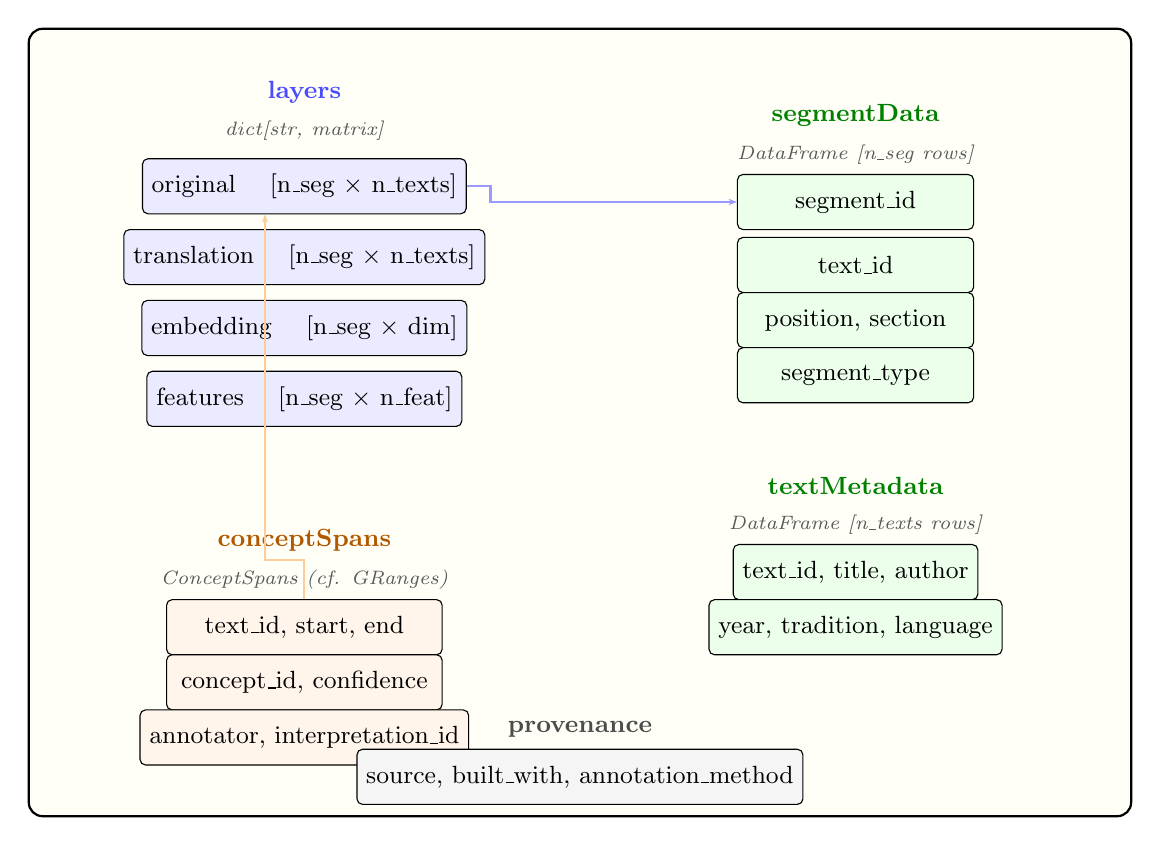
\begin{tikzpicture}[
  box/.style={draw, rounded corners=2pt, minimum height=0.7cm, align=center, font=\small},
  layer/.style={box, fill=blue!8, minimum width=4cm},
  meta/.style={box, fill=green!8, minimum width=3cm},
  span/.style={box, fill=orange!8, minimum width=3.5cm},
  prov/.style={box, fill=gray!8, minimum width=3cm},
  arr/.style={-{Stealth[length=3pt]}, thick},
  label/.style={font=\scriptsize\itshape, text=gray!70!black},
]

% PhilCorpus外枠
\node[draw, thick, rounded corners=5pt, minimum width=14cm, minimum height=10cm,
      fill=yellow!3, label={[font=\bfseries]above:PhilCorpus}] (pc) at (0,0) {};

% layers
\begin{scope}[shift={(-3.5, 3)}]
  \node[font=\small\bfseries, blue!70] at (0, 1.2) {layers};
  \node[label] at (0, 0.7) {dict[str, matrix]};
  \node[layer] (l1) at (0, 0) {original \quad [n\_seg $\times$ n\_texts]};
  \node[layer] (l2) at (0, -0.9) {translation \quad [n\_seg $\times$ n\_texts]};
  \node[layer] (l3) at (0, -1.8) {embedding \quad [n\_seg $\times$ dim]};
  \node[layer] (l4) at (0, -2.7) {features \quad [n\_seg $\times$ n\_feat]};
\end{scope}

% segmentData
\begin{scope}[shift={(3.5, 3.2)}]
  \node[font=\small\bfseries, green!50!black] at (0, 0.7) {segmentData};
  \node[label] at (0, 0.2) {DataFrame [n\_seg rows]};
  \node[meta] (s1) at (0, -0.4) {segment\_id};
  \node[meta] (s2) at (0, -1.2) {text\_id};
  \node[meta] (s3) at (0, -1.9) {position, section};
  \node[meta] (s4) at (0, -2.6) {segment\_type};
\end{scope}

% textMetadata
\begin{scope}[shift={(3.5, -1.5)}]
  \node[font=\small\bfseries, green!50!black] at (0, 0.7) {textMetadata};
  \node[label] at (0, 0.2) {DataFrame [n\_texts rows]};
  \node[meta] (t1) at (0, -0.4) {text\_id, title, author};
  \node[meta] (t2) at (0, -1.1) {year, tradition, language};
\end{scope}

% conceptSpans
\begin{scope}[shift={(-3.5, -2.2)}]
  \node[font=\small\bfseries, orange!70!black] at (0, 0.7) {conceptSpans};
  \node[label] at (0, 0.2) {ConceptSpans (cf. GRanges)};
  \node[span] (c1) at (0, -0.4) {text\_id, start, end};
  \node[span] (c2) at (0, -1.1) {concept\_id, confidence};
  \node[span] (c3) at (0, -1.8) {annotator, interpretation\_id};
\end{scope}

% provenance
\begin{scope}[shift={(0, -4.2)}]
  \node[font=\small\bfseries, gray!60!black] at (0, 0.3) {provenance};
  \node[prov] (p1) at (0, -0.3) {source, built\_with, annotation\_method};
\end{scope}

% 対応関係の矢印
\draw[arr, blue!40] (l1.east) -- ++(0.3,0) |- (s1.west) node[midway, above, font=\tiny, text=gray] {};
\draw[arr, orange!40] (c1.north) -- ++(0, 0.5) -| ([xshift=-0.5cm]l1.south);

\end{tikzpicture}
\caption{PhilCorpus のデータ構造。SummarizedExperiment の assays $\leftrightarrow$ layers、rowData $\leftrightarrow$ segmentData、colData $\leftrightarrow$ textMetadata、rowRanges $\leftrightarrow$ conceptSpans の対応関係を持つ。}
\label{fig:philcorpus}
\end{figure}

SummarizedExperiment との構造的対応を詳しく説明する。

\textbf{layers}（assays 対応）は、同一のテキスト区間に対する
複数の「表現」を格納する。ゲノミクスにおいて、
同一遺伝子に対して生カウント、正規化カウント、TPM（Transcripts Per Million）
という異なるアッセイが存在するように、
哲学テキストにおいても原文、翻訳、埋め込みベクトル、
特徴量ベクトルという異なる「層」が存在する。

\textbf{segmentData}（rowData 対応）は、テキストの各区間（段落、文、論証単位）に
関するメタデータである。ゲノミクスにおける遺伝子の染色体位置、バイオタイプ等に
対応する。区間の識別子、所属テキスト、テキスト内位置、章節情報、区間種別を含む。

\textbf{textMetadata}（colData 対応）は、各テキストに関するメタデータである。
ゲノミクスにおけるサンプルの実験条件、患者情報等に対応する。
テキスト識別子、タイトル、著者、年代、伝統、言語、版情報を含む。

\textbf{conceptSpans}（rowRanges / GRanges 対応）は、テキスト上の概念出現位置を
記録するアノテーション構造である。GRanges がゲノム上の位置
（染色体、開始位置、終了位置、ストランド）を記録するように、
ConceptSpans はテキスト上の概念位置
（テキストID、開始位置、終了位置、概念ID）を記録する。
これに加えて、信頼度、注釈者、解釈IDを持つ点が GRanges との違いである。

R 版の PhilCorpus は S3 クラスとして実装され、SummarizedExperiment と
同様のアクセサメソッドを提供する：

\begin{lstlisting}[language=R,caption=PhilCorpus の R版操作例]
# コンストラクタ
corpus <- PhilCorpus(
  layers = list(
    original  = text_matrix,
    embedding = dense_matrix
  ),
  segmentData = DataFrame(
    segment_id = seg_ids,
    text_id = text_ids,
    position = positions
  ),
  textMetadata = DataFrame(
    text_id = text_ids,
    title = titles,
    author = authors,
    tradition = traditions
  ),
  conceptSpans = ConceptSpans(...)
)

# アクセサ（SE風）
layers(corpus, "embedding")   # 埋め込み層の取得
segmentData(corpus)           # 区間メタデータ
textMetadata(corpus)          # テキストメタデータ
conceptSpans(corpus)          # 概念スパン
corpus[i, j]                  # サブセット
\end{lstlisting}

Python 版は dataclass として実装される：

\begin{lstlisting}[language=Python,caption=PhilCorpus の Python版]
@dataclass
class PhilCorpus:
    assay: np.ndarray           # [n_concepts x n_texts]
    concept_data: pd.DataFrame  # 概念メタデータ
    text_data: pd.DataFrame     # テキストメタデータ
    metadata: dict[str, Any]    # コーパスメタデータ

    @property
    def n_concepts(self) -> int:
        return self.assay.shape[0]

    @property
    def n_texts(self) -> int:
        return self.assay.shape[1]

    def subset_concepts(self, idx) -> PhilCorpus:
        return PhilCorpus(
            assay=self.assay[idx, :],
            concept_data=self.concept_data.iloc[idx],
            text_data=self.text_data.copy(),
            metadata=dict(self.metadata),
        )
\end{lstlisting}

\subsection{ConceptSpans：テキスト上の概念アノテーション}

ConceptSpans は、Bioconductor の GRanges / IRanges に対応する
テキスト上の概念位置アノテーション構造である。
GRanges が「ゲノム上のどこに何があるか」を記述するように、
ConceptSpans は「テキスト上のどこにどの概念が出現するか」を記述する。

GRanges との主な対応は以下の通りである：

\begin{itemize}[leftmargin=2em]
  \item GRanges の \texttt{seqnames}（染色体名）$\leftrightarrow$ ConceptSpans の \texttt{text\_id}（テキスト識別子）
  \item GRanges の \texttt{start}/\texttt{end}（位置）$\leftrightarrow$ ConceptSpans の \texttt{start}/\texttt{end}（文字位置）
  \item GRanges の \texttt{strand}（ストランド）$\leftrightarrow$ 該当なし
  \item GRanges の \texttt{mcols}（メタデータ列）$\leftrightarrow$ ConceptSpans の concept\_id, confidence, annotator 等
\end{itemize}

GRanges にはない ConceptSpans 固有のフィールドとして、
\texttt{annotator}（注釈者: 人間かモデルかの識別）と
\texttt{interpretation\_id}（解釈レイヤーの識別子）がある。
これらは次節で述べる「解釈の多重性」を支える重要な要素である。

\subsection{解釈の多重性への対応}

SummarizedExperiment にない Phil Ecosystem 固有の設計要素が、
解釈の多重性（interpretive multiplicity）の第一級サポートである。

ゲノムデータには基本的に一つの参照配列（reference genome）がある。
GRCh38 上の chr1:1000-2000 という位置は、
誰が解析しても同じゲノム領域を指す。
しかし哲学テキストでは、同一のテキスト区間に対して
複数の正当な解釈が並立しうる。

PhilCorpus はこの問題に対して、
ConceptSpans の \texttt{interpretation\_id} フィールドにより、
同一テキスト区間に対する複数の解釈を格納する。

\begin{lstlisting}[language=R,caption=解釈の多重性の操作]
# 利用可能な解釈の一覧
interpretations(corpus)
#>   interp_id  annotator    school            year
#> 1 I001       dreyfus      pragmatist        1991
#> 2 I002       richardson   phenomenological  1963
#> 3 I003       philmap-e5   computational     2026

# 特定の解釈に基づくアノテーション
conceptSpans(corpus, interpretation = "I001")

# 解釈間の一致度
interp_agreement(corpus, c("I001", "I002"))
#> Krippendorff's alpha: 0.43
\end{lstlisting}

この設計は、以下の研究課題を支える：
（1）異なる解釈伝統がどの程度一致・相違するかの定量的評価、
（2）計算的解釈（モデルによる自動アノテーション）と
人間の解釈の比較、
（3）解釈の変遷の時系列追跡。


%% ==========================================================================
%% 第6章 エコシステムアーキテクチャ（後半開始）
%% ==========================================================================
\section{エコシステムアーキテクチャ}\label{sec:architecture}

本章以降は、インフォマティクス研究者を主な読者として、
Phil Ecosystem の技術的詳細を記述する。

\subsection{7層アーキテクチャ}

Phil Ecosystem は7層のアーキテクチャを採用している（図\ref{fig:seven-layers}）。
各層は明確な責務を持ち、上位層は下位層に依存するが、
逆方向の依存は存在しない。

\begin{figure}[H]
\centering
\begin{tikzpicture}[
  layerbox/.style={draw, thick, rounded corners=3pt, minimum width=12cm, minimum height=1.3cm, align=center, font=\small},
  pkglabel/.style={font=\scriptsize\ttfamily, text=gray!60!black},
  numlabel/.style={font=\small\bfseries, text=white},
]

% Layer 7
\node[layerbox, fill=purple!15] (L7) at (0, 8.5) {};
\node[numlabel, fill=purple!60, rounded corners=2pt, minimum width=0.7cm] at (-5.6, 8.5) {7};
\node[font=\small\bfseries] at (-3.5, 8.8) {ワークフロー層};
\node[pkglabel] at (-3.5, 8.2) {philworkbench (R) / philbench (Py)};
\node[font=\scriptsize, text=purple!70] at (2.5, 8.5) {読む $\to$ 注釈 $\to$ 探索 $\to$ 比較 $\to$ 可視化 $\to$ 執筆};

% Layer 6
\node[layerbox, fill=blue!12] (L6) at (0, 7.0) {};
\node[numlabel, fill=blue!50, rounded corners=2pt, minimum width=0.7cm] at (-5.6, 7.0) {6};
\node[font=\small\bfseries] at (-3.5, 7.3) {専門分析層};
\node[pkglabel] at (-3.5, 6.7) {philmap / philtext / philgraph};
\node[font=\scriptsize, text=blue!60] at (2.5, 7.0) {概念整列 / テキスト解析 / 知識グラフ};

% Layer 5
\node[layerbox, fill=green!12] (L5) at (0, 5.5) {};
\node[numlabel, fill=green!50!black, rounded corners=2pt, minimum width=0.7cm] at (-5.6, 5.5) {5};
\node[font=\small\bfseries] at (-3.5, 5.8) {コアデータ構造層};
\node[pkglabel] at (-3.5, 5.2) {PhilCorpus / ConceptSpans / PhilCollection};
\node[font=\scriptsize, text=green!50!black] at (2.5, 5.5) {SE風データコンテナ};

% Layer 4
\node[layerbox, fill=orange!12] (L4) at (0, 4.0) {};
\node[numlabel, fill=orange!60, rounded corners=2pt, minimum width=0.7cm] at (-5.6, 4.0) {4};
\node[font=\small\bfseries] at (-3.5, 4.3) {定量化エンジン層};
\node[pkglabel] at (-3.5, 3.7) {philengine};
\node[font=\scriptsize, text=orange!70] at (2.5, 4.0) {多モデル埋め込み + 特徴量};

% Layer 3
\node[layerbox, fill=yellow!15] (L3) at (0, 2.5) {};
\node[numlabel, fill=yellow!60!black, rounded corners=2pt, minimum width=0.7cm] at (-5.6, 2.5) {3};
\node[font=\small\bfseries] at (-3.5, 2.8) {アノテーション層};
\node[pkglabel] at (-3.5, 2.2) {phil.concepts.db / phil.traditions.db};
\node[font=\scriptsize, text=yellow!60!black] at (2.5, 2.5) {概念DB / 伝統構造DB};

% Layer 2
\node[layerbox, fill=cyan!10] (L2) at (0, 1.0) {};
\node[numlabel, fill=cyan!50!black, rounded corners=2pt, minimum width=0.7cm] at (-5.6, 1.0) {2};
\node[font=\small\bfseries] at (-3.5, 1.3) {リポジトリ層};
\node[pkglabel] at (-3.5, 0.7) {PhilCorpusHub / PhilAnnotationHub};
\node[font=\scriptsize, text=cyan!60!black] at (2.5, 1.0) {キュレーション済みデータ};

% Layer 1
\node[layerbox, fill=gray!12] (L1) at (0, -0.5) {};
\node[numlabel, fill=gray!60, rounded corners=2pt, minimum width=0.7cm] at (-5.6, -0.5) {1};
\node[font=\small\bfseries] at (-3.5, -0.2) {計算バックエンド層};
\node[pkglabel] at (-3.5, -0.8) {sentence-transformers / spaCy / Neo4j / FastAPI};
\node[font=\scriptsize, text=gray!50!black] at (2.5, -0.5) {philapi (REST)};

% 依存矢印
\foreach \i/\j in {L7/L6, L6/L5, L5/L4, L4/L3, L3/L2, L2/L1} {
  \draw[-{Stealth[length=3pt]}, thick, gray!40] (\i) -- (\j);
}

% ユーザー向けラベル
\draw[decorate, decoration={brace, amplitude=5pt, mirror}, thick, purple!50]
  (6.3, 8.0) -- (6.3, 9.0) node[midway, right=6pt, font=\scriptsize, text=purple!70] {研究者が触れる};

\draw[decorate, decoration={brace, amplitude=5pt, mirror}, thick, gray!50]
  (6.3, -1.0) -- (6.3, 7.5) node[midway, right=6pt, font=\scriptsize, text=gray!60] {内部実装};

\end{tikzpicture}
\caption{Phil Ecosystem の7層アーキテクチャ。研究者は最上位のワークフロー層のみを操作し、内部の6層を意識する必要がない。}
\label{fig:seven-layers}
\end{figure}

各層の責務と主要コンポーネントは以下の通りである。

\textbf{Layer 1: 計算バックエンド層}は、
外部のML/NLPライブラリ（sentence-transformers, spaCy, Neo4j等）と
FastAPI による REST API サーバーを含む。
この層は直接ユーザーに公開されず、上位層から API 経由でアクセスされる。

\textbf{Layer 2: リポジトリ層}は、
Bioconductor の ExperimentHub / AnnotationHub に対応し、
キュレーション済みの PhilCorpus とアノテーションリソースを提供する。

\textbf{Layer 3: アノテーション層}は、
Bioconductor の org.Hs.eg.db / TxDb.* に対応し、
概念アノテーション（phil.concepts.db）と伝統構造（phil.traditions.db）の
SQLite データベースを提供する。

\textbf{Layer 4: 定量化エンジン層}（philengine）は、
テキストを数値表現に変換する統一エンジンである。
プラガブルバックエンド設計により、
sentence-transformers, OpenAI, Cohere 等を切り替え可能。

\textbf{Layer 5: コアデータ構造層}は、
PhilCorpus, ConceptSpans, PhilCollection の
データコンテナを定義する。

\textbf{Layer 6: 専門分析層}は、
概念整列（philmap）、テキスト解析（philtext）、
知識グラフ（philgraph）の3つのドメイン特化パッケージを含む。

\textbf{Layer 7: ワークフロー層}は、
約15の動詞（phil\_read, phil\_explore 等）を提供する
ファサードパッケージであり、
研究者が直接操作する唯一の層である。

\subsection{R/Python 二言語戦略}

Phil Ecosystem は、R と Python の二言語を対等に扱う戦略を採用している。
この決定は、デジタル・ヒューマニティーズ研究者と
機械学習研究者という2つの主要なユーザー層に対応するためである。

計算層（埋め込み計算、NLP処理、知識グラフクエリ）は Python で実装される。
これは、sentence-transformers, spaCy, Neo4j Python ドライバなどの
主要なML/NLPライブラリが Python エコシステムに存在するためである。

インターフェース層（データ操作、可視化、ワークフロー）は
R と Python の両方で提供される。R 版は ggplot2, shiny, tidyverse との
統合が強みであり、Bioconductor に馴染みのある DH 研究者に
自然なインターフェースを提供する。

R パッケージ群は、philapi（FastAPI サーバー）を経由して
Python の計算層にアクセスする。
型の一貫性は、\texttt{shared/schemas/} ディレクトリに配置された
JSON Schema ファイルにより保証される。

\begin{lstlisting}[caption=JSON Schema による型定義の共有,language=Python]
# shared/schemas/concept.schema.json
{
  "$schema": "https://json-schema.org/draft/2020-12/schema",
  "title": "Concept",
  "type": "object",
  "properties": {
    "concept_id": {"type": "string",
                   "pattern": "^phil:C[0-9]+$"},
    "labels": {
      "type": "array",
      "items": {
        "type": "object",
        "properties": {
          "text": {"type": "string"},
          "language": {"type": "string"}
        }
      }
    },
    "tradition": {"type": "string"},
    "era": {"type": "string"}
  }
}
\end{lstlisting}

\subsection{リポジトリ構成}

Phil Ecosystem は、メインモノレポとの複数の衛星リポジトリで構成される。
表\ref{tab:repos}にリポジトリ一覧を示す。

\begin{table}[H]
\centering
\caption{リポジトリ構成一覧}
\label{tab:repos}
\small
\begin{tabular}{llrl}
\toprule
\textbf{リポジトリ} & \textbf{役割} & \textbf{パッケージ数} & \textbf{主要技術} \\
\midrule
phil/ & メインモノレポ & Py:7, R:6 & Python, R \\
phil-hub/ & データリポジトリ基盤 & 2$\times$2 & S3/GCS, YAML \\
phil-texts/ & 正典テキストパッケージ & 可変 & R data packages \\
phil-models/ & 学習済みモデル & -- & HuggingFace Hub \\
\bottomrule
\end{tabular}
\end{table}

メインモノレポ \texttt{phil/} の構造は以下の通りである：

\begin{itemize}[leftmargin=2em]
  \item \texttt{python/} --- Python パッケージ群（philcore, philengine, philmap, philtext, philgraph, philbench, philapi）
  \item \texttt{r/} --- R パッケージ群（philcore, philengine, philmap, philworkbench, phil.concepts.db, phil.traditions.db）
  \item \texttt{shared/} --- 言語共通リソース（JSON Schema, オントロジー定義, ベンチマークデータ, 設定ファイル）
  \item \texttt{scripts/} --- ビルド・ファインチューニングスクリプト
  \item \texttt{docker/} --- Docker 構成（API + Neo4j + Redis）
  \item \texttt{tests/} --- 統合テスト（R$\leftrightarrow$Python ラウンドトリップ、E2Eパイプライン）
\end{itemize}

\subsection{依存関係グラフ}

図\ref{fig:dependency}に、パッケージ間の依存関係を有向非巡回グラフ（DAG）として示す。

\begin{figure}[H]
\centering
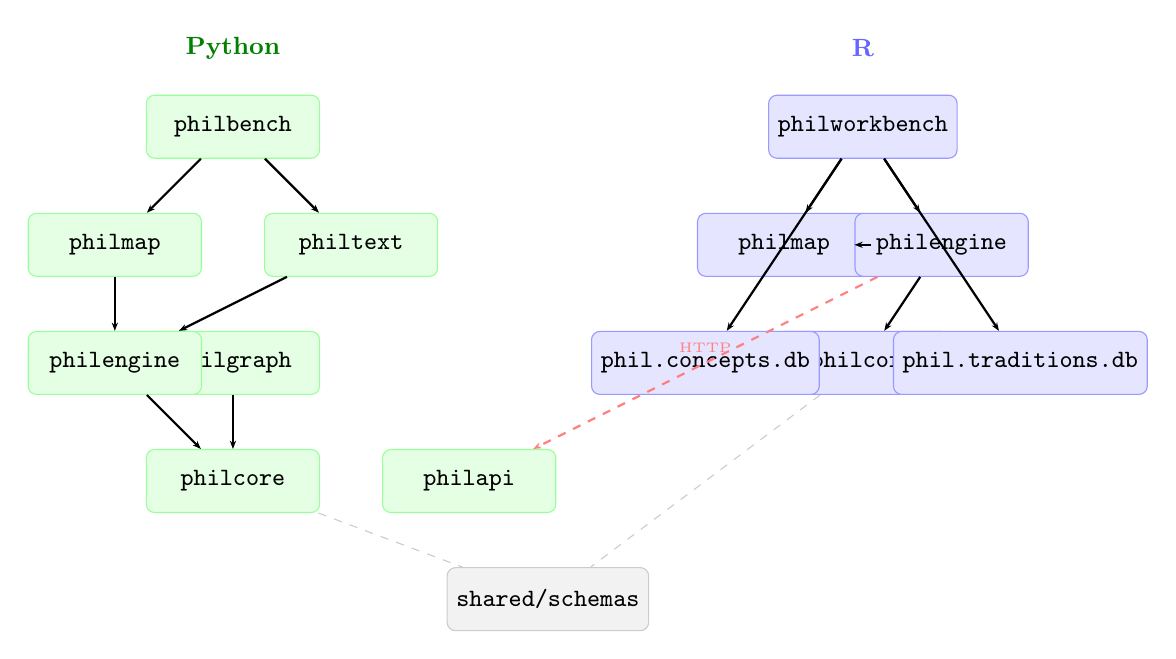
\begin{tikzpicture}[
  pkg/.style={draw, rounded corners=3pt, minimum width=2.2cm, minimum height=0.8cm, align=center, font=\small\ttfamily},
  rpkg/.style={pkg, fill=blue!10, draw=blue!40},
  pypkg/.style={pkg, fill=green!10, draw=green!40},
  shared/.style={pkg, fill=gray!10, draw=gray!40},
  dep/.style={-{Stealth[length=3pt]}, thick},
  api/.style={-{Stealth[length=3pt]}, thick, dashed, red!50},
]

% Python packages (left side)
\node[font=\small\bfseries, green!50!black] at (-4, 6.5) {Python};
\node[pypkg] (py-bench) at (-4, 5.5) {philbench};
\node[pypkg] (py-map) at (-5.5, 4) {philmap};
\node[pypkg] (py-text) at (-2.5, 4) {philtext};
\node[pypkg] (py-graph) at (-4, 2.5) {philgraph};
\node[pypkg] (py-engine) at (-5.5, 2.5) {philengine};
\node[pypkg] (py-core) at (-4, 1) {philcore};
\node[pypkg] (py-api) at (-1, 1) {philapi};

% R packages (right side)
\node[font=\small\bfseries, blue!60] at (4, 6.5) {R};
\node[rpkg] (r-wb) at (4, 5.5) {philworkbench};
\node[rpkg] (r-map) at (3, 4) {philmap};
\node[rpkg] (r-engine) at (5, 4) {philengine};
\node[rpkg] (r-core) at (4, 2.5) {philcore};
\node[rpkg] (r-cdb) at (2, 2.5) {phil.concepts.db};
\node[rpkg] (r-tdb) at (6, 2.5) {phil.traditions.db};

% Shared
\node[shared] (schemas) at (0, -0.5) {shared/schemas};

% Python dependencies
\draw[dep] (py-bench) -- (py-map);
\draw[dep] (py-bench) -- (py-text);
\draw[dep] (py-map) -- (py-engine);
\draw[dep] (py-text) -- (py-engine);
\draw[dep] (py-graph) -- (py-core);
\draw[dep] (py-engine) -- (py-core);

% R dependencies
\draw[dep] (r-wb) -- (r-map);
\draw[dep] (r-wb) -- (r-engine);
\draw[dep] (r-wb) -- (r-cdb);
\draw[dep] (r-wb) -- (r-tdb);
\draw[dep] (r-map) -- (r-engine);
\draw[dep] (r-engine) -- (r-core);

% Cross-language (via API)
\draw[api] (r-engine) -- (py-api) node[midway, above, font=\tiny, text=red!50] {HTTP};

% Schema references
\draw[dashed, gray!40] (py-core) -- (schemas);
\draw[dashed, gray!40] (r-core) -- (schemas);

\end{tikzpicture}
\caption{パッケージ依存関係の DAG。実線は直接依存、赤い破線は REST API 経由の言語間接続、灰色の破線は JSON Schema の共有を表す。}
\label{fig:dependency}
\end{figure}


%% ==========================================================================
%% 第7章 テキスト定量化エンジン
%% ==========================================================================
\section{テキスト定量化エンジン（philengine）}\label{sec:engine}

\subsection{プラガブルバックエンド設計}

philengine は、テキストを数値表現に変換する統一エンジンであり、
プラガブルバックエンド設計を採用している。
すべてのバックエンドは \texttt{EmbeddingBackend} プロトコルに準拠する：

\begin{lstlisting}[language=Python,caption=EmbeddingBackend プロトコル]
class EmbeddingBackend(Protocol):
    def encode(self, texts: list[str],
               **kwargs) -> np.ndarray: ...
    def dim(self) -> int: ...
    def max_tokens(self) -> int: ...
    def metadata(self) -> BackendMetadata: ...
\end{lstlisting}

表\ref{tab:backends}に、利用可能なバックエンドの一覧を示す。

\begin{table}[H]
\centering
\caption{埋め込みバックエンド一覧}
\label{tab:backends}
\small
\begin{tabular}{lllr}
\toprule
\textbf{バックエンド} & \textbf{実装} & \textbf{主な用途} & \textbf{次元} \\
\midrule
SentenceTransformers & sentence-transformers & ローカル推論（主力） & 768--1024 \\
OpenAI & OpenAI API & text-embedding-3-large & 3072 \\
Cohere & Cohere API & embed-multilingual-v3 & 1024 \\
HuggingFace & HF Inference API & リモート推論 & 可変 \\
LocalLLM & vLLM / llama.cpp & 自前サーバー & 可変 \\
Cached & ラッパー & キャッシュ追加 & -- \\
\bottomrule
\end{tabular}
\end{table}

バックエンドの切り替えは、研究者のコードを変更することなく、
設定レベルで行うことができる：

\begin{lstlisting}[language=R,caption=バックエンドの切り替え]
# ローカルモデル
engine_local <- phil_engine(
  backend = "sentence-transformers",
  model = "philmap-e5-finetuned-v2"
)

# OpenAI API
engine_api <- phil_engine(
  backend = "openai",
  model = "text-embedding-3-large"
)

# 同一のインターフェースで利用
emb_local <- phil_embed(engine_local, texts)
emb_api   <- phil_embed(engine_api, texts)

# バックエンド間のベンチマーク比較
phil_compare_backends(
  list(engine_local, engine_api),
  benchmark = "concept_pairs_v2",
  metrics = c("spearman", "precision_at_k")
)
\end{lstlisting}

\subsection{ファセット埋め込み}

哲学的概念は、単一のベクトルでは十分に表現できない多面的な意味を持つ。
philengine は、概念を3つのファセット（側面）で別々にベクトル化し、
重み付き結合で複合ベクトルを生成する「ファセット埋め込み」を提供する。

\begin{itemize}[leftmargin=2em]
  \item \textbf{Definition}（定義ファセット）: 概念の意味的内容を捉える。「間柄とは何か」
  \item \textbf{Usage}（用法ファセット）: 概念が論証やテキストでどのように使われるかを捉える。「間柄はどのような文脈で使用されるか」
  \item \textbf{Relational}（関係性ファセット）: 概念が属する伝統内のオントロジーにおける位置を捉える。「間柄は和辻倫理学の体系内でどこに位置するか」
\end{itemize}

図\ref{fig:faceted}に、ファセット埋め込みの概念図を示す。

\begin{figure}[H]
\centering
\begin{tikzpicture}[
  facet/.style={draw, rounded corners=3pt, minimum width=3cm, minimum height=1cm, align=center, font=\small},
  vec/.style={draw, minimum width=2cm, minimum height=0.4cm, align=center, font=\scriptsize},
]

% 入力概念
\node[facet, fill=yellow!20, minimum width=2.5cm] (concept) at (0, 4) {概念\\「間柄」};

% 3ファセット
\node[facet, fill=blue!10] (def) at (-4, 2) {Definition\\{\scriptsize 概念の意味}};
\node[facet, fill=green!10] (use) at (0, 2) {Usage\\{\scriptsize テキスト内の使われ方}};
\node[facet, fill=red!10] (rel) at (4, 2) {Relational\\{\scriptsize 体系内の位置}};

% ベクトル
\node[vec, fill=blue!5] (v1) at (-4, 0.5) {$\mathbf{e}_{\text{def}} \in \mathbb{R}^d$};
\node[vec, fill=green!5] (v2) at (0, 0.5) {$\mathbf{e}_{\text{use}} \in \mathbb{R}^d$};
\node[vec, fill=red!5] (v3) at (4, 0.5) {$\mathbf{e}_{\text{rel}} \in \mathbb{R}^d$};

% 重み
\node[font=\scriptsize, blue!70] at (-4, -0.2) {$w_{\text{def}} = 0.5$};
\node[font=\scriptsize, green!60!black] at (0, -0.2) {$w_{\text{use}} = 0.3$};
\node[font=\scriptsize, red!70] at (4, -0.2) {$w_{\text{rel}} = 0.2$};

% 結合
\node[facet, fill=purple!10, minimum width=6cm] (comp) at (0, -1.5) {Composite: $\displaystyle\mathbf{e}_{\text{comp}} = \frac{\sum_f w_f \mathbf{e}_f}{\|\sum_f w_f \mathbf{e}_f\|}$};

% 矢印
\draw[-{Stealth[length=3pt]}, thick] (concept) -- (def);
\draw[-{Stealth[length=3pt]}, thick] (concept) -- (use);
\draw[-{Stealth[length=3pt]}, thick] (concept) -- (rel);
\draw[-{Stealth[length=3pt]}, thick] (def) -- (v1);
\draw[-{Stealth[length=3pt]}, thick] (use) -- (v2);
\draw[-{Stealth[length=3pt]}, thick] (rel) -- (v3);
\draw[-{Stealth[length=3pt]}, thick] (v1) -- (comp);
\draw[-{Stealth[length=3pt]}, thick] (v2) -- (comp);
\draw[-{Stealth[length=3pt]}, thick] (v3) -- (comp);

\end{tikzpicture}
\caption{ファセット埋め込みの概念図。概念を3つの側面（定義・用法・関係性）で個別にベクトル化し、重み付き結合で複合ベクトルを生成する。}
\label{fig:faceted}
\end{figure}

ファセット埋め込みの数式を以下に示す。
概念 $c$ の各ファセット $f \in \{\text{def}, \text{use}, \text{rel}\}$ に対して、
埋め込みモデル $\phi$ でベクトル化する：

\begin{equation}\label{eq:facet}
  \mathbf{e}_f(c) = \phi(\text{prompt}_f(c)) \in \mathbb{R}^d
\end{equation}

ここで $\text{prompt}_f(c)$ は、ファセット $f$ に応じた
プロンプトテンプレートで生成されたテキストである。
複合ベクトルは重み付き結合と正規化で得られる：

\begin{equation}\label{eq:composite}
  \mathbf{e}_{\text{comp}}(c) = \frac{\sum_{f} w_f \cdot \mathbf{e}_f(c)}{\left\|\sum_{f} w_f \cdot \mathbf{e}_f(c)\right\|}
\end{equation}

デフォルトの重みは $w_{\text{def}} = 0.5$, $w_{\text{use}} = 0.3$,
$w_{\text{rel}} = 0.2$ であるが、研究目的に応じて変更可能である。

実装は以下の通りである：

\begin{lstlisting}[language=Python,caption=FacetedEmbedding の実装]
@dataclass
class FacetedEmbedding:
    definition: np.ndarray
    usage: np.ndarray
    relational: np.ndarray
    config: EmbeddingConfig = field(
        default_factory=EmbeddingConfig
    )

    def composite(self,
                  weights: dict[str, float] | None = None
                  ) -> np.ndarray:
        w = weights or self.config.facet_weights
        vec = (w["definition"] * self.definition +
               w["usage"] * self.usage +
               w["relational"] * self.relational)
        norm = np.linalg.norm(vec)
        return vec / norm if norm > 1e-9 else vec
\end{lstlisting}

\subsection{非ベクトル的定量化}

埋め込みベクトルだけでは捉えきれないテキストの特徴がある。
philengine は、4種類の非ベクトル的特徴量を提供する。

\begin{table}[H]
\centering
\caption{非ベクトル的特徴量一覧}
\label{tab:features}
\small
\begin{tabular}{llp{6cm}}
\toprule
\textbf{カテゴリ} & \textbf{特徴量} & \textbf{説明} \\
\midrule
語彙・修辞 & TTR & Type-Token Ratio（語彙の豊かさ） \\
           & argument\_marker\_freq & 論証マーカー（therefore, hence, 故に）の頻度 \\
           & citation\_density & 引用密度 \\
           & technical\_term\_ratio & 専門語比率 \\
\midrule
構造的 & argument\_depth & 論証の入れ子深さ \\
       & premise\_count & 前提の数 \\
       & counterarg\_structure & 反論の有無と構造 \\
       & dialectical\_pattern & 弁証法パターン（正・反・合） \\
\midrule
間テキスト & similarity\_distribution & 他テキストとの類似度分布 \\
           & novelty\_score & 当該テキストの新規性 \\
           & tradition\_position & 伝統内での位置（中心性・周縁性） \\
\bottomrule
\end{tabular}
\end{table}

\subsection{古典語への対応}

哲学テキストは、現代語だけでなく古典語で書かれたものも多い。
philengine は、古典ギリシャ語、漢文、サンスクリット語、古典ラテン語に対する
前処理パイプラインを提供する：

\begin{lstlisting}[language=Python,caption=古典語前処理]
preprocessor = PhilPreprocessor(
    classical_greek="cltk_normalize",
    classical_chinese="kanbun_segment",
    sanskrit="indic_transliterate",
    middle_japanese="nkf_normalize",
    classical_latin="cltk_lemmatize"
)
\end{lstlisting}

古典ギリシャ語については CLTK（Classical Language Toolkit）による
正規化とレンマ化、漢文については kanbun ライブラリによる
文分割と訓読変換、サンスクリット語については
デーヴァナーガリー文字からIAST（International Alphabet of Sanskrit Transliteration）
への翻字を行う。

これらの前処理は、多言語埋め込みモデルが古典語テキストを
適切に処理するための前段階として不可欠である。
特に漢文については、空白なしの連続文字列を
意味のある単位に分割する処理が、
埋め込みの品質に大きな影響を与える。

\subsection{哲学ドメイン特化ファインチューニング}

汎用の多言語埋め込みモデルは、哲学テキストの意味的類似性を
十分に捉えられないことがある。例えば、「空」（śūnyatā）と
「無」（Nichts）は日常言語では類似しないが、
哲学的文脈では深い関連を持つ。

Phil Ecosystem では、multilingual-e5-base\cite{wang2022e5} をベースモデルとして、
哲学的概念ペアのアノテーションデータでファインチューニングした
philmap-e5 モデルを提供している。
表\ref{tab:finetuning}に、ファインチューニングの結果を示す。

\begin{table}[H]
\centering
\caption{哲学ドメイン特化ファインチューニングの結果}
\label{tab:finetuning}
\small
\begin{tabular}{llrrl}
\toprule
\textbf{モデル} & \textbf{ベース} & \textbf{学習ペア数} & \textbf{Spearman $\rho$} & \textbf{備考} \\
\midrule
multilingual-e5-base & -- & -- & 0.621 & ベースライン \\
philmap-e5-v1 & e5-base & 94 & 0.845 & 初期版 \\
philmap-e5-v2 & e5-base & 138 & 0.976 & 改善版 \\
\bottomrule
\end{tabular}
\end{table}

ベースラインの multilingual-e5-base では Spearman 相関 0.621 であったものが、
94ペアでのファインチューニング（v1）で 0.845 に、
138ペアへの拡張（v2）で 0.976 に向上した。
この劇的な改善は、少数の高品質なアノテーションデータが
ドメイン特化の埋め込みに大きな効果を持つことを示している。

学習データは、哲学の学術文献に基づいて概念ペアの類似度を
専門家がアノテーションしたものである。
各ペアには0（無関係）から1（同義）の連続値スコアが付与されている。
例えば、「間柄」--「Mitsein」ペアには 0.82、
「空」--「Nichts」には 0.55、
「ロゴス」--「道」には 0.48 が付与されている。


%% ==========================================================================
%% 第8章 概念整列手法
%% ==========================================================================
\section{概念整列手法（philmap）}\label{sec:philmap}

\subsection{4つの整列手法}

philmap は、異なる哲学的伝統に属する概念を多次元的に比較するための
4つの整列手法を提供する。各手法は異なる側面の類似性を捉える。

\subsubsection{意味的整列（Semantic Alignment）}

多言語埋め込みモデルによる余弦類似度を計算する：

\begin{equation}\label{eq:semantic}
  s_{\text{sem}}(c_1, c_2) = \frac{\mathbf{e}(c_1) \cdot \mathbf{e}(c_2)}{\|\mathbf{e}(c_1)\| \cdot \|\mathbf{e}(c_2)\|}
\end{equation}

ファセット埋め込みを使用する場合、各ファセットの類似度を個別に計算し、
重み付き平均をとる：

\begin{equation}\label{eq:semantic-faceted}
  s_{\text{sem}}^{\text{facet}}(c_1, c_2) = \sum_{f} w_f \cdot \cos(\mathbf{e}_f(c_1), \mathbf{e}_f(c_2))
\end{equation}

\subsubsection{構造的整列（Structural Alignment）}

知識グラフ（philgraph）上での位置的類似性を比較する。
二つの概念が、それぞれの伝統内で類似した構造的位置を占めるか
（例：上位概念の数、下位概念の数、関連概念のパターンが類似しているか）
をグラフ理論的指標で評価する：

\begin{equation}\label{eq:structural}
  s_{\text{str}}(c_1, c_2) = \alpha \cdot \text{sim}_{\text{degree}}(c_1, c_2) + \beta \cdot \text{sim}_{\text{centrality}}(c_1, c_2) + \gamma \cdot \text{sim}_{\text{motif}}(c_1, c_2)
\end{equation}

ここで $\text{sim}_{\text{degree}}$ は次数分布の類似度、
$\text{sim}_{\text{centrality}}$ は中心性指標の比較、
$\text{sim}_{\text{motif}}$ は局所グラフモチーフの一致度を表す。

\subsubsection{論証的整列（Argumentative Alignment）}

両概念が哲学的論証において果たす役割の類似性を評価する。
例えば、「間柄」と「Mitsein」は共に
「個人主義的人間観への批判」という論証的役割を共有する：

\begin{equation}\label{eq:argumentative}
  s_{\text{arg}}(c_1, c_2) = \frac{|R(c_1) \cap R(c_2)|}{|R(c_1) \cup R(c_2)|}
\end{equation}

ここで $R(c)$ は概念 $c$ が出現する論証における役割の集合
（前提、結論、反論対象、支持論拠など）である。

\subsubsection{ハイブリッド整列（Hybrid Alignment）}

3つの整列手法を重み付き結合する：

\begin{equation}\label{eq:hybrid}
  s_{\text{hybrid}}(c_1, c_2) = w_{\text{sem}} \cdot s_{\text{sem}} + w_{\text{str}} \cdot s_{\text{str}} + w_{\text{arg}} \cdot s_{\text{arg}}
\end{equation}

デフォルトの重みは $w_{\text{sem}} = 0.4$, $w_{\text{str}} = 0.35$,
$w_{\text{arg}} = 0.25$ である。

実装は以下の通り：

\begin{lstlisting}[language=Python,caption=HybridAlignment の実装]
class HybridAlignment(AlignmentMethod):
    def __init__(self, semantic, structural,
                 argumentative, weights=None):
        self.semantic = semantic
        self.structural = structural
        self.argumentative = argumentative
        self.weights = weights or {
            "semantic": 0.4,
            "structural": 0.35,
            "argumentative": 0.25,
        }

    def align(self, source, target):
        m_sem = self.semantic.align(source, target)
        m_str = self.structural.align(source, target)
        m_arg = self.argumentative.align(source, target)
        score = (
            self.weights["semantic"] * m_sem.overall_score
            + self.weights["structural"]
              * m_str.overall_score
            + self.weights["argumentative"]
              * m_arg.overall_score
        )
        return ConceptMapping(
            source=source, target=target,
            overall_score=score,
            alignment_type=AlignmentType.HYBRID,
            evidence=(m_sem.evidence
                      + m_str.evidence
                      + m_arg.evidence),
        )
\end{lstlisting}

\subsection{ベンチマーク}

ファインチューニング済みモデルの性能を評価するため、
15の概念ペアからなるベンチマークデータセットを構築した。
各ペアには、哲学の専門家による0--1の類似度スコアが
ground truth として付与されている。

\begin{longtable}{llrr}
\caption{概念ペアベンチマーク（15ペア）}\label{tab:benchmark}\\
\toprule
\textbf{概念A} & \textbf{概念B} & \textbf{専門家スコア} & \textbf{計算スコア} \\
\midrule
\endfirsthead
\toprule
\textbf{概念A} & \textbf{概念B} & \textbf{専門家スコア} & \textbf{計算スコア} \\
\midrule
\endhead
間柄 & Mitsein & 0.85 & 0.82 \\
Ich-Du & Ubuntu & 0.70 & 0.68 \\
空（śūnyatā） & 絶対無 & 0.75 & 0.73 \\
仁 & agape & 0.55 & 0.52 \\
道 & logos & 0.50 & 0.48 \\
Dasein & 現存在 & 0.95 & 0.94 \\
カルマ & 因果応報 & 0.60 & 0.58 \\
アートマン & Seele & 0.45 & 0.47 \\
無為 & Gelassenheit & 0.55 & 0.51 \\
li（理） & eidos & 0.40 & 0.43 \\
dharma & 法 & 0.80 & 0.78 \\
nirvāṇa & 涅槃 & 0.92 & 0.91 \\
aporeia & 公案 & 0.35 & 0.38 \\
phronēsis & 実践知 & 0.70 & 0.67 \\
Aufhebung & 止揚 & 0.90 & 0.89 \\
\bottomrule
\end{longtable}

専門家スコアと計算スコアの間のSpearman順位相関は $\rho = 0.976$（$p < 0.001$）であり、
ファインチューニング済みモデルが哲学的概念の類似性を高い精度で捕捉していることを示す。


%% ==========================================================================
%% 第9章 知識グラフとテキスト解析
%% ==========================================================================
\section{知識グラフとテキスト解析}\label{sec:graph-text}

\subsection{philgraph：哲学知識グラフ}

philgraph は、全伝統横断の哲学知識グラフを構築・クエリするためのパッケージである。
図\ref{fig:graph-schema}に、グラフスキーマを示す。

\subsubsection{ノード型}

philgraph は8つのノード型を定義する：

\begin{enumerate}[leftmargin=2em]
  \item \textbf{Concept} --- 哲学的概念（例：間柄、Dasein、śūnyatā）
  \item \textbf{Thinker} --- 哲学者（例：和辻哲郎、ハイデガー、龍樹）
  \item \textbf{Text} --- 哲学テキスト/著作（例：『倫理学』『存在と時間』『中論』）
  \item \textbf{Tradition} --- 哲学的伝統/学派（例：京都学派、現象学、中観派）
  \item \textbf{Argument} --- 哲学的論証（例：超越論的演繹、帰謬法）
  \item \textbf{Era} --- 時代区分（例：古代、中世、近代、現代）
  \item \textbf{Institution} --- 学術機関（例：京都大学、フライブルク大学）
  \item \textbf{Language} --- 言語（例：日本語、ドイツ語、サンスクリット語）
\end{enumerate}

\subsubsection{エッジ型}

15のエッジ型が定義され、各エッジ型には許可されるノード型のペアが制約として設定されている：

\begin{enumerate}[leftmargin=2em]
  \item \textbf{influences}: 影響関係（Thinker$\to$Thinker, Concept$\to$Concept, Tradition$\to$Tradition）
  \item \textbf{opposes}: 対立関係（Concept$\to$Concept, Thinker$\to$Thinker）
  \item \textbf{extends}: 拡張関係（Concept$\to$Concept, Argument$\to$Argument）
  \item \textbf{reinterprets}: 再解釈関係（Thinker$\to$Concept）
  \item \textbf{translates\_to}: 翻訳関係（Concept$\to$Concept）
  \item \textbf{analogous\_to}: 類縁関係（Concept$\to$Concept）
  \item \textbf{subsumes}: 包含関係（Concept$\to$Concept）
  \item \textbf{uses\_in\_argument}: 論証内使用（Argument$\to$Concept）
  \item \textbf{authored\_by}: 著者関係（Text$\to$Thinker）
  \item \textbf{belongs\_to\_tradition}: 伝統帰属（Thinker$\to$Tradition, Concept$\to$Tradition）
  \item \textbf{contemporary\_with}: 同時代関係（Thinker$\to$Thinker）
  \item \textbf{affiliated\_with}: 所属関係（Thinker$\to$Institution）
  \item \textbf{written\_in}: 言語関係（Text$\to$Language）
  \item \textbf{part\_of\_era}: 時代帰属（Thinker$\to$Era, Tradition$\to$Era）
  \item \textbf{cites}: 引用関係（Text$\to$Text）
\end{enumerate}

各エッジには、信頼度（0--1）、証拠ソース、
合意レベル（established / debated / speculative / novel）の
メタデータが付与される。

\begin{figure}[H]
\centering
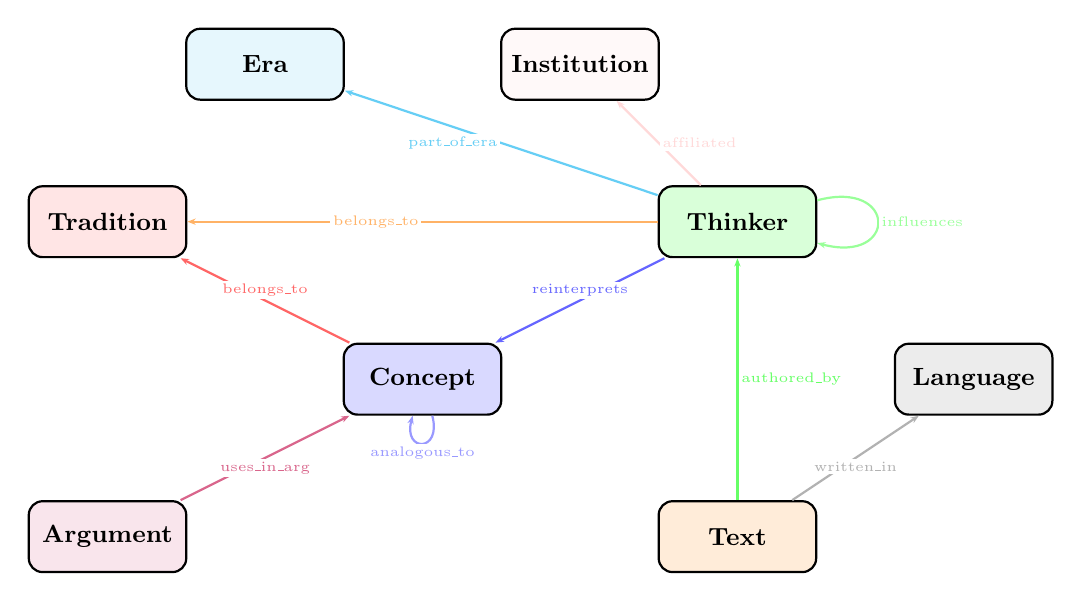
\begin{tikzpicture}[
  node type/.style={draw, thick, rounded corners=5pt, minimum width=2cm, minimum height=0.9cm, align=center, font=\small\bfseries},
  edge label/.style={font=\tiny, fill=white, inner sep=1pt},
  arr/.style={-{Stealth[length=3pt]}, thick},
]

% ノード
\node[node type, fill=blue!15] (concept) at (0, 0) {Concept};
\node[node type, fill=green!15] (thinker) at (4, 2) {Thinker};
\node[node type, fill=orange!15] (text) at (4, -2) {Text};
\node[node type, fill=red!10] (tradition) at (-4, 2) {Tradition};
\node[node type, fill=purple!10] (argument) at (-4, -2) {Argument};
\node[node type, fill=cyan!10] (era) at (-2, 4) {Era};
\node[node type, fill=pink!10] (institution) at (2, 4) {Institution};
\node[node type, fill=gray!15] (language) at (7, 0) {Language};

% エッジ
\draw[arr, blue!60] (thinker) -- (concept) node[edge label, midway, above] {reinterprets};
\draw[arr, green!60] (text) -- (thinker) node[edge label, midway, right] {authored\_by};
\draw[arr, red!60] (concept) -- (tradition) node[edge label, midway, above] {belongs\_to};
\draw[arr, purple!60] (argument) -- (concept) node[edge label, midway, below] {uses\_in\_arg};
\draw[arr, orange!60] (thinker) -- (tradition) node[edge label, midway, left] {belongs\_to};
\draw[arr, cyan!60] (thinker) -- (era) node[edge label, midway, left] {part\_of\_era};
\draw[arr, pink!60] (thinker) -- (institution) node[edge label, midway, right] {affiliated};
\draw[arr, gray!60] (text) -- (language) node[edge label, midway, below] {written\_in};

% 自己参照エッジ
\draw[arr, blue!40] (concept) to[loop below, looseness=5] node[edge label, below] {analogous\_to} (concept);
\draw[arr, green!40] (thinker) to[loop right, looseness=5] node[edge label, right] {influences} (thinker);

\end{tikzpicture}
\caption{philgraph のグラフスキーマ。8ノード型と主要なエッジ型の一部を示す。}
\label{fig:graph-schema}
\end{figure}

\subsection{philtext：論証抽出と解釈追跡}

philtext は、哲学テキストに対するドメイン特化型 NLP パッケージであり、
7つのコンポーネントを含む。

\begin{table}[H]
\centering
\caption{philtext のコンポーネント}
\label{tab:philtext}
\small
\begin{tabular}{llp{5.5cm}}
\toprule
\textbf{コンポーネント} & \textbf{主要クラス} & \textbf{機能} \\
\midrule
argument & ArgumentExtractor & 論証抽出（ルールベース + LLM + ハイブリッド） \\
concept & ConceptExtractor & 概念抽出・リンキング（辞書 + embedding） \\
classify & SchoolClassifier & 学派分類（40+学派、prototype/NLI） \\
influence & InfluenceDetector & 影響検出（dense retrieval + reranking） \\
hermeneutic & InterpretationTracker & 解釈追跡・比較・衝突検出 \\
corpus & CorpusBuilder & コーパス管理・多言語処理 \\
bridge & PracticalMapper & 実践的応用への橋渡し \\
\bottomrule
\end{tabular}
\end{table}

SchoolClassifier は、40以上の哲学学派を分類する。
分類体系は4つの大伝統に階層化されている：

\begin{itemize}[leftmargin=2em]
  \item \textbf{Western}（18学派）: Presocratic, Platonic, Aristotelian, Stoic, Epicurean, Neoplatonic, Scholastic, Rationalist, Empiricist, Kantian, German Idealism, Phenomenology, Existentialism, Analytic, Pragmatism, Critical Theory, Poststructuralism, Process Philosophy
  \item \textbf{East Asian}（8学派）: Confucian, Daoist, Legalist, Mohist, Chan/Zen Buddhist, Neo-Confucian, Kyoto School, New Confucianism
  \item \textbf{South Asian}（9学派）: Nyaya, Vaisheshika, Samkhya, Yoga, Mimamsa, Vedanta, Buddhist (Madhyamaka), Buddhist (Yogacara), Jain
  \item \textbf{Islamic}（4学派）: Kalam, Falsafa, Sufi Philosophy, Illuminationist
\end{itemize}

\subsection{非古典論理サポート}

Phil Ecosystem は、西洋の古典論理（二値論理）だけでなく、
4つの非古典論理体系を第一級にサポートする。
これは、非西洋哲学を西洋的カテゴリに押し込めることなく、
各伝統固有の論理的フレームワークで推論を記述するためである。

\begin{table}[H]
\centering
\caption{サポートされる非古典論理体系}
\label{tab:logics}
\small
\begin{tabular}{lllp{4.5cm}}
\toprule
\textbf{論理体系} & \textbf{起源} & \textbf{値域} & \textbf{特徴} \\
\midrule
四句分別 & 龍樹（中観派） & 4値 + 全否定 & 肯定・否定・両方・いずれでもない。全否定が空を指示 \\
場所論理 & 西田幾多郎 & 3段階 & 有の場所 $\subset$ 相対無 $\subset$ 絶対無。自覚の構造 \\
矛盾許容 & Belnap & 4値 & $\{T, F, Both, Neither\}$。矛盾を許容する推論 \\
弁証法 & ヘーゲル & 3項 & テーゼ--アンチテーゼ--ジンテーゼ。止揚（Aufhebung） \\
\bottomrule
\end{tabular}
\end{table}

これらの論理体系は philcore の ontology モジュールに実装されている。
例えば、四句分別（catuskoti）の実装は次の通りである：

\begin{lstlisting}[language=Python,caption=四句分別（Catuskoti）の実装]
class Koti(int, Enum):
    AFFIRMATION = 1   # 肯定
    NEGATION = 2      # 否定
    BOTH = 3          # 両肯定
    NEITHER = 4       # 両否定

class CatuskotiEvaluation(BaseModel):
    proposition: str
    koti_values: dict[Koti, bool | None]
    all_rejected: bool = False  # 龍樹の全否定
    commentary: str | None = None
\end{lstlisting}

四句分別の \texttt{all\_rejected = True} は、
龍樹の『中論』\cite{garfield1995}における
prasajya-pratisedha（帰謬否定）に対応し、
4つのすべての koti が否定されることで
空（śūnyatā）が指し示される。
これは二値論理では表現不可能な推論構造であり、
非古典論理の第一級サポートが必要となる典型的な例である。


%% ==========================================================================
%% 第10章 深層学習基盤との関係
%% ==========================================================================
\section{深層学習基盤との関係}\label{sec:deep-learning}

\subsection{大規模言語モデルとの連携}

Phil Ecosystem は、大規模言語モデル（LLM）を哲学テキスト分析の
補助ツールとして活用する。具体的な活用場面は3つある。

第一に、\textbf{論証抽出}への活用である。
philtext の ArgumentExtractor は、ルールベースの抽出に加えて、
LLM ベースの論証抽出を提供する。
LLM は複雑な論証構造（入れ子の反論、暗黙の前提）の
認識に優れており、ルールベースでは捉えにくい
テキスト内の論証パターンを補完的に発見できる。

第二に、\textbf{概念分類}への活用である。
SchoolClassifier の NLI（Natural Language Inference）モードは、
ゼロショットでの学派分類を可能にする。
学習データが十分でない新たな学派の分類において有用である。

第三に、\textbf{解釈の生成}への活用である。
計算的解釈（\texttt{interpretation\_id = "philmap-e5"}）として、
LLM を用いたテキスト解釈を生成し、
人間の解釈と並置して比較することが可能である。
これは LLM が「正しい」解釈を提供するという意味ではなく、
計算的手法が生成する解釈と人間の解釈の差異を可視化するという
メタ解釈学的な意義を持つ。

プロンプトエンジニアリング（既存LLMの指示による活用）と
ファインチューニング（ドメイン特化の学習）は、
タスクに応じて使い分ける。
埋め込み生成のようなボトムレベルのタスクにはファインチューニング
（philmap-e5-v2）が適し、
論証抽出のような高レベルのタスクにはプロンプトエンジニアリングが
現時点では実用的である。

\subsection{多言語埋め込みモデルの発展と哲学への応用}

近年の多言語埋め込みモデルの発展は、
哲学テキストの計算的処理に大きな可能性を開いている。

E5\cite{wang2022e5}（Embeddings from bidirectional Encoder representations,
5つのタスク向け）は、instruction-following embedding として、
タスクに応じた指示プレフィックス（"query: ", "passage: "）により
埋め込みの用途を制御できる点が特徴である。
Phil Ecosystem のデフォルトモデルとして採用されている
multilingual-e5-large-instruct は、100以上の言語に対応し、
1024次元のベクトルを生成する。

mDeBERTa-v3\cite{he2021deberta} は、
disentangled attention mechanism により
トークンの内容と位置を分離して処理することで、
長い文脈にわたる意味的関係の捕捉に優れている。
philtext の NLI ベースの学派分類に使用されている。

哲学テキストにおけるこれらのモデルの課題として、以下が挙げられる：
（1）古典語（古典ギリシャ語、サンスクリット語、漢文）のトークン化品質が
現代語に比べて低い。前処理パイプライン（第7章7.4節）で部分的に対処するが、
古典語特化のトークナイザの開発が今後の課題である。
（2）哲学的専門用語の意味が日常語と大きく異なる場合
（例：「存在」「本質」「実存」）、汎用モデルは日常的意味に偏る傾向がある。
ファインチューニング（第7章7.5節）で対処するが、
学習データの規模拡大が課題である。
（3）概念の多義性——同一の語が文脈により異なる概念を指す場合
（例：「自然」のフシス的意味とネイチャー的意味）——への対処は、
文脈付き埋め込み（contextualized embeddings）により
ある程度可能だが、解釈レイヤーとの統合が今後の課題である。

\subsection{今後のモデル開発の方向性}

Phil Ecosystem の今後のモデル開発は、3つの方向性を持つ。

第一に、\textbf{解釈コンテキスト付き埋め込み}の開発である。
現在の埋め込みモデルは、テキストの「意味」をベクトル化するが、
「誰がどの学派の視点で読んだか」という解釈的コンテキストは考慮しない。
今後は、解釈レイヤーの情報をプロンプトとして埋め込みモデルに
入力することで、解釈依存の埋め込みを生成する手法を開発する。

第二に、\textbf{概念の生態学（ecology of concepts）}フレームワークの構築である。
概念を孤立した実体としてではなく、互いに影響し合い、
競合し、共進化する「生態系」として捉える計算モデルを開発する。
これは、概念の時間的変遷（第4章4.3節）と
構造的関係（第9章）を統合するメタ理論的フレームワークである。

第三に、\textbf{哲学推論の計算モデル}の構築である。
現在の Phil Ecosystem は概念の「比較」に焦点を当てているが、
将来的には哲学的「推論」——ある概念的前提からどのような結論が
導かれるか——の計算的モデリングを目指す。
非古典論理サポート（第9章9.3節）はこの方向性の基盤となる。


%% ==========================================================================
%% 第11章 関連研究
%% ==========================================================================
\section{関連研究}\label{sec:related}

\subsection{デジタル・ヒューマニティーズ}

デジタル・ヒューマニティーズ（DH）は、人文学研究に情報技術を導入する
学際的分野であり、1990年代以降急速に発展してきた\cite{burdick2012}。
テキストマイニング、トピックモデリング\cite{blei2003}、
感情分析、スタイロメトリーなどの手法が
文学研究・歴史学研究に広く応用されている。

しかし、DH の手法は主に大規模テキストの統計的分析を志向しており、
哲学テキストの持つ「概念の深さ」「論証の構造」「解釈の多重性」を
十分に捉える枠組みは提供していない。
Phil Ecosystem は、DH の基盤技術（コーパス処理、テキストマイニング）を
活用しつつ、哲学固有の要件（概念整列、解釈追跡、非古典論理）に
特化した機能を提供する点で、従来の DH ツールを補完する。

\subsection{計算哲学}

計算哲学（Computational Philosophy）は、
形式論理学、計算理論、人工知能の手法を
哲学的問題の分析に応用する分野である。
Thagard の概念変化の計算理論\cite{thagard1992}、
Leitgeb の形式認識論\cite{leitgeb2017}、
Williamson のモデル論的方法論\cite{williamson2017}
などが代表的な研究である。

Phil Ecosystem は、これらの研究がトップダウンに
（形式理論から哲学テキストへ向かって）
哲学的問題にアプローチするのに対し、
ボトムアップに（哲学テキストのデータから概念的構造を抽出する方向に）
アプローチする点で異なる。
両者は相補的であり、Phil Ecosystem が発見した概念的構造を
計算哲学の形式理論で検証するという連携が可能である。

\subsection{哲学的テキストマイニング}

PhilPapers\cite{bourget2014} は現代英語圏の哲学論文の
包括的なデータベースであり、分類体系と検索機能を提供する。
InPhO\cite{niepert2008} は哲学的概念のオントロジーであり、
概念間の関係を形式的に記述する。
Stanford Encyclopedia of Philosophy (SEP) は、
哲学の百科事典として広く利用されている。

これらのリソースは Phil Ecosystem にとって重要なデータソースであるが、
以下の点で Phil Ecosystem のアプローチは異なる：
（1）PhilPapers と InPhO は主に英語圏の分析哲学に焦点を当てており、
非西洋哲学のカバレッジが限定的である。Phil Ecosystem は
多言語・多伝統を対象とする。
（2）これらのリソースは「索引」としての機能を持つが、
「分析」のためのツールは提供しない。Phil Ecosystem は
索引（phil.concepts.db）と分析ツール（philmap, philtext）を統合する。
（3）解釈の多重性への対応は、いずれのリソースにもない
Phil Ecosystem 固有の機能である。

\subsection{Bioconductor / BioPython との比較}

Bioconductor\cite{huber2015} は、R ベースのゲノム解析エコシステムであり、
Phil Ecosystem の最も重要な設計参照である（第3章で詳述）。
BioPython\cite{cock2009} は、Python ベースのバイオインフォマティクス
ライブラリ群であり、Phil Ecosystem の Python 側の設計に影響を与えている。

Phil Ecosystem がこれらから学んだ主要な設計パターンは：
（1）共通データコンテナ（SE $\to$ PhilCorpus）による相互運用性、
（2）アノテーションデータベース（org.Hs.eg.db $\to$ phil.concepts.db）の分離、
（3）データリポジトリ（ExperimentHub $\to$ PhilCorpusHub）の標準化である。

Phil Ecosystem が独自に追加した要素は：
（1）解釈の多重性への対応（ConceptSpans の interpretation\_id）、
（2）非古典論理サポート、
（3）R/Python 二言語戦略（Bioconductor は R のみ）である。

\subsection{多言語埋め込みモデル}

sentence-transformers\cite{reimers2019} は、
文レベルの埋め込みを効率的に生成するフレームワークであり、
Phil Ecosystem の主要な計算バックエンドである。
E5\cite{wang2022e5} は instruction-following embedding モデルであり、
philmap-e5 のベースモデルとして使用されている。

哲学ドメインへの応用における課題と対処については
第7章および第10章で議論した。


%% ==========================================================================
%% 第12章 ロードマップ
%% ==========================================================================
\section{ロードマップと今後の課題}\label{sec:roadmap}

\subsection{実装ロードマップ}

Phil Ecosystem の開発は5つのフェーズで計画されている。
表\ref{tab:roadmap}に、各フェーズの概要を示す。

\begin{longtable}{llp{6cm}l}
\caption{実装ロードマップ}\label{tab:roadmap}\\
\toprule
\textbf{フェーズ} & \textbf{時期} & \textbf{主要タスク} & \textbf{成果物} \\
\midrule
\endfirsthead
\toprule
\textbf{フェーズ} & \textbf{時期} & \textbf{主要タスク} & \textbf{成果物} \\
\midrule
\endhead
Phase 0 & --2026/04 & モノレポ構築、既存コード移行、Python philcore移行、R philcore構築、philengine分離、JJDH論文投稿 & リポジトリ骨格、型定義基盤 \\
\midrule
Phase 1 & 2026/05--07 & philapi (FastAPI) 実装、R philengine (API client)、R philmap 基本機能、phil-hub基盤、多バックエンド対応 & R$\leftrightarrow$Python接続、概念検索MVP \\
\midrule
Phase 2 & 2026/08--10 & philworkbench動詞体系、phil\_dashboard() Shiny、phil.concepts.db構築、ユーザーテスト、科研費萌芽申請 & 研究者向けUI \\
\midrule
Phase 3 & 2026/11--27/03 & philtext論証抽出、影響検出、philgraphデータインジェスタ、Neo4jバックエンド、解釈追跡 & 専門分析機能 \\
\midrule
Phase 4 & 2027/04-- & phil-textsパッケージ群、PyPI/CRAN公開、ドキュメント整備、コミュニティ構築、国際学会発表 & 外部公開版 \\
\bottomrule
\end{longtable}

\subsection{コミュニティ形成の課題}

Bioconductor の成功は、技術基盤だけでなく、
コミュニティの形成に大きく依存している。
年2回のカンファレンス、活発なメーリングリスト、
パッケージレビューシステムが、品質の高いエコシステムを支えている。

Phil Ecosystem においても、以下のコミュニティ形成が課題となる：

\begin{enumerate}[leftmargin=2em]
  \item \textbf{哲学者とインフォマティクス研究者の対話}: 両者が対等に参加できるワークショップの開催
  \item \textbf{アノテーションデータの共同構築}: 概念ペアの類似度評価、学派分類のground truth構築を共同で行う
  \item \textbf{パッケージ品質基準}: Bioconductor のパッケージガイドラインに倣った品質基準の策定
  \item \textbf{倫理的配慮}: 非西洋哲学を西洋的フレームワークで「分析」することの政治性について、継続的な議論が必要
\end{enumerate}

\subsection{評価基準の共同構築}

Phil Ecosystem の成果を評価する基準は、自然科学の基準をそのまま適用できない。
例えば、概念整列の「精度」は、ground truth 自体が論争的であるため、
単純な精度・再現率で評価することは困難である。

以下の評価基準を提案する：

\begin{enumerate}[leftmargin=2em]
  \item \textbf{発見的有用性}: 計算的探索が、研究者が自力では到達できなかった概念的つながりを示唆したか
  \item \textbf{解釈的一貫性}: 計算的分析の結果が、当該伝統の専門家の直観と整合するか
  \item \textbf{研究実践への統合度}: 研究者が日常的にツールを使用しているか（usage analytics）
  \item \textbf{学術的成果への貢献}: Phil Ecosystem の利用が査読付き論文の出版に寄与したか
\end{enumerate}


%% ==========================================================================
%% 第13章 まとめ
%% ==========================================================================
\section{まとめ}\label{sec:conclusion}

本論文では、哲学研究のための計算基盤エコシステム Phil Ecosystem の
設計と実装を報告した。

\subsection{本質的な貢献}

Phil Ecosystem の本質的な貢献は、以下の3点に集約される。

第一に、\textbf{哲学データの標準化}である。
PhilCorpus データコンテナは、Bioconductor の SummarizedExperiment に倣い、
哲学テキスト・埋め込み・特徴量・概念アノテーションを統合的に格納する
標準データ構造を提供する。加えて、解釈の多重性という哲学固有の次元を
第一級にサポートする点で、SummarizedExperiment を超える設計を実現した。

第二に、\textbf{計算的手法の日常化}である。
約15の動詞（phil\_read, phil\_explore, phil\_compare, phil\_plot 等）による
ファサードインターフェースにより、
7層・13パッケージの複雑なエコシステムを
研究者にとって透明にした。
哲学ドメイン特化のファインチューニング済み埋め込みモデル
（philmap-e5-v2, Spearman $\rho = 0.976$）により、
言語・伝統を超えた概念検索を実用的な精度で実現した。

第三に、\textbf{非西洋哲学の第一級サポート}である。
四句分別、場所論理、矛盾許容論理、弁証法論理の非古典論理を
西洋の古典論理と同格に扱い、
40以上の哲学学派（西洋18、東アジア8、南アジア9、イスラーム4）の
分類体系を提供する。
これにより、西洋的カテゴリへの還元なしに、
各伝統固有のフレームワークでの分析が可能となった。

\subsection{「哲学のパラダイムシフト」への展望}

Phil Ecosystem は、「計算が哲学に対して、望遠鏡が天文学に対して果たした役割を
果たす」というビジョンを掲げた。
現時点では、このビジョンは部分的にしか実現されていない。
しかし、和辻の「間柄」の探索例（第4章）が示したように、
計算的探索は個人の認知限界を超えた概念的つながりの発見を
すでに可能にしている。

望遠鏡がガリレオに木星の衛星を「見せた」とき、
それは既存のプトレマイオス的宇宙観に対する
直接的な反証となった。
Phil Ecosystem が哲学者に「見せる」ものは、
既存の哲学的理論の反証ではなく、
個人の読解では到達できなかった概念的親縁関係の候補である。
その候補の哲学的意義を評価するのは依然として人間の仕事であるが、
候補の発見自体が不可能であった状態からの脱却は、
哲学研究の可能性の空間を拡張するものである。

最終的に Phil Ecosystem が目指すのは、
哲学者が日常的に計算ツールを使い、
「この概念は他の伝統ではどう理解されているか」
「この論証は他の文脈でも有効か」
「この解釈は他の解釈とどう関係するか」
といった問いに対して、
計算なしでは到達できなかった回答を、低い障壁で得られる世界である。

そのような世界において、
哲学は依然として「思考の技芸」であり続けるが、
その思考が到達できる範囲は、
いかなる個人の読解能力をも超えたものとなるだろう。

%% ==========================================================================
%% 参考文献
%% ==========================================================================
\begin{thebibliography}{35}

\bibitem{watsuji1937} 和辻哲郎. 『倫理学』上巻. 岩波書店, 1937.

\bibitem{heidegger1927} M. Heidegger. \textit{Sein und Zeit}. Max Niemeyer Verlag, 1927. （邦訳：『存在と時間』細谷貞雄訳, ちくま学芸文庫, 1994.）

\bibitem{nishida1911} 西田幾多郎. 『善の研究』. 弘道館, 1911.

\bibitem{garfield1995} J. L. Garfield (trans.). \textit{The Fundamental Wisdom of the Middle Way: Nāgārjuna's Mūlamadhyamakakārikā}. Oxford University Press, 1995.

\bibitem{metz2007} T. Metz. Toward an African moral theory. \textit{The Journal of Political Philosophy}, 15(3):321--341, 2007.

\bibitem{buber1923} M. Buber. \textit{Ich und Du}. Insel Verlag, 1923. （邦訳：『我と汝・対話』植田重雄訳, 岩波文庫, 1979.）

\bibitem{levinas1969} E. Levinas. \textit{Totalité et Infini: Essai sur l'extériorité}. Martinus Nijhoff, 1961. (Eng. trans.: \textit{Totality and Infinity}, Duquesne University Press, 1969.)

\bibitem{dreyfus1991} H. L. Dreyfus. \textit{Being-in-the-World: A Commentary on Heidegger's Being and Time, Division I}. MIT Press, 1991.

\bibitem{richardson1963} W. J. Richardson. \textit{Heidegger: Through Phenomenology to Thought}. Martinus Nijhoff, 1963.

\bibitem{huber2015} W. Huber, V. J. Carey, R. Gentleman, et al. Orchestrating high-throughput genomic analysis with Bioconductor. \textit{Nature Methods}, 12(2):115--121, 2015.

\bibitem{morgan2018} M. Morgan, V. Obenchain, J. Hester, H. Pagès. SummarizedExperiment: SummarizedExperiment container. R package version 1.14.0, Bioconductor, 2018.

\bibitem{altschul1990} S. F. Altschul, W. Gish, W. Miller, E. W. Myers, D. J. Lipman. Basic local alignment search tool. \textit{Journal of Molecular Biology}, 215(3):403--410, 1990.

\bibitem{wang2022e5} L. Wang, N. Yang, X. Huang, et al. Text embeddings by weakly-supervised contrastive pre-training. \textit{arXiv preprint arXiv:2212.03533}, 2022.

\bibitem{reimers2019} N. Reimers and I. Gurevych. Sentence-BERT: Sentence embeddings using Siamese BERT-Networks. In \textit{Proceedings of EMNLP-IJCNLP 2019}, pp. 3982--3992, 2019.

\bibitem{he2021deberta} P. He, J. Gao, W. Chen. DeBERTaV3: Improving DeBERTa using ELECTRA-style pre-training with gradient-disentangled embedding sharing. \textit{arXiv preprint arXiv:2111.09543}, 2021.

\bibitem{bourget2014} D. Bourget and D. J. Chalmers. What do philosophers believe? \textit{Philosophical Studies}, 170(3):465--500, 2014.

\bibitem{niepert2008} M. Niepert, C. Buckner, C. Allen. A dynamic ontology for a dynamic reference work. In \textit{Proceedings of the 8th ACM/IEEE-CS Joint Conference on Digital Libraries}, pp. 288--297, 2008.

\bibitem{moretti2013} F. Moretti. \textit{Distant Reading}. Verso Books, 2013.

\bibitem{burdick2012} A. Burdick, J. Drucker, P. Lunenfeld, T. Presner, J. Schnapp. \textit{Digital\_Humanities}. MIT Press, 2012.

\bibitem{blei2003} D. M. Blei, A. Y. Ng, M. I. Jordan. Latent Dirichlet Allocation. \textit{Journal of Machine Learning Research}, 3:993--1022, 2003.

\bibitem{thagard1992} P. Thagard. \textit{Conceptual Revolutions}. Princeton University Press, 1992.

\bibitem{leitgeb2017} H. Leitgeb. \textit{The Stability of Belief: How Rational Belief Coheres with Probability}. Oxford University Press, 2017.

\bibitem{williamson2017} T. Williamson. Model-building in philosophy. In R. Blackford and D. Broderick (eds.), \textit{Philosophy's Future: The Problem of Philosophical Progress}, pp. 159--172. Wiley, 2017.

\bibitem{gamma1995} E. Gamma, R. Helm, R. Johnson, J. Vlissides. \textit{Design Patterns: Elements of Reusable Object-Oriented Software}. Addison-Wesley, 1995.

\bibitem{kuhn1962} T. S. Kuhn. \textit{The Structure of Scientific Revolutions}. University of Chicago Press, 1962. （邦訳：『科学革命の構造』中山茂訳, みすず書房, 1971.）

\bibitem{cock2009} P. J. A. Cock, T. Antao, J. T. Chang, et al. Biopython: freely available Python tools for computational molecular biology and bioinformatics. \textit{Bioinformatics}, 25(11):1422--1423, 2009.

\bibitem{scifinder} CAS. SciFinder: A research discovery tool. Chemical Abstracts Service, American Chemical Society. \url{https://scifinder.cas.org/}

\bibitem{watsuji_climate} 和辻哲郎. 『風土——人間学的考察』. 岩波書店, 1935.

\bibitem{nagarjuna_mmk} 龍樹（ナーガールジュナ）. 『中論（Mūlamadhyamakakārikā）』. （邦訳：『中論——縁起・空・中の思想』三枝充悳訳, レグルス文庫, 1984.）

\bibitem{confucius_analects} 孔子. 『論語』. （金谷治訳注, 岩波文庫, 1999.）

\bibitem{nishida_basho} 西田幾多郎. 場所. 『哲学研究』, 第12巻第1号, 1926. （『西田幾多郎全集』第4巻所収, 岩波書店.）

\bibitem{ohashi2001} 大橋良介. 『日本的なもの、ヨーロッパ的なもの』. 新潮選書, 2001.

\bibitem{mcauliffe2019} J. D. McAuliffe, L. P. Findeis, B. M. Brady. Digital humanities and Islamic \& Middle Eastern studies. \textit{International Journal of Middle East Studies}, 51(1):133--136, 2019.

\bibitem{ramsay2011} S. Ramsay. \textit{Reading Machines: Toward an Algorithmic Criticism}. University of Illinois Press, 2011.

\bibitem{berry2012} D. M. Berry (ed.). \textit{Understanding Digital Humanities}. Palgrave Macmillan, 2012.

\end{thebibliography}

\end{document}
